\documentclass[12pt,spanish,fleqn,openany,letterpaper,pagesize]{scrbook}

\usepackage[utf8]{inputenc}
\usepackage[spanish]{babel}
\usepackage{fancyhdr}
\usepackage{epsfig}
\usepackage{epic}
\usepackage{eepic}
\usepackage{amsmath}

\usepackage{amsthm}

\usepackage{nccmath}
\usepackage{threeparttable}
\usepackage{amscd}
\usepackage{here}
\usepackage{graphicx}
\usepackage{lscape}
\usepackage{tabularx}
\usepackage{subfigure}
\usepackage{longtable}
\usepackage{paralist}
\usepackage{blkarray}

% Me
\usepackage{multicol}
\setlength{\columnseprule}{0.4pt}

\usepackage{tikz}
\usepackage[hidelinks]{hyperref}
\usepackage{siunitx}
\usepackage{stanli}

\usepackage{listings}
\usepackage{color}
\usepackage{breakcites}

\usepackage[style=apa,citestyle=apa]{biblatex}
\DefineBibliographyStrings{spanish}{%
  andothers = {et al}
  }
\addbibresource{BibliMSc.bib}

\usepackage{nicematrix}
% \usepackage{titlesec}

\usepackage{tikz-imagelabels}
\imagelabelset{
	outer dist = -0.5 cm
}

\usepackage{dirtree}

\theoremstyle{plain}
\newtheorem{example}{Ejemplo}[chapter]

\usepackage{caption}

\renewcommand{\lstlistingname}{Algoritmo}% Listing -> Algorithm
\renewcommand{\lstlistlistingname}{Lista de \lstlistingname s}% List of Listings -> List of Algorithm

%New colors defined below
\definecolor{codegreen}{rgb}{0,0.6,0}
\definecolor{codegray}{rgb}{0.5,0.5,0.5}
\definecolor{codepurple}{rgb}{0.58,0,0.82}
\definecolor{backcolour}{rgb}{0.95,0.95,0.92}

%Code listing style named "mystyle"
\lstdefinestyle{mystyle}{
%   backgroundcolor=\color{backcolour},   commentstyle=\color{codegreen},
  keywordstyle=\color{magenta},
  numberstyle=\tiny\color{codegray},
  stringstyle=\color{codepurple},
  basicstyle=\footnotesize,
  breakatwhitespace=false,         
  breaklines=true,                 
  captionpos=top,                    
  keepspaces=true,                 
%   numbers=left,                    
  numbersep=5pt,                  
  showspaces=false,                
  showstringspaces=false,
  showtabs=false,                  
  tabsize=2
}

%"mystyle" code listing set
\lstset{style=mystyle}

% Formato de definiciones y ejemplos 
\usepackage[listingsutf8,breakable,many]{tcolorbox}
% \tcbuselibrary{minted}

% Caja sin título
\newtcolorbox{cajasimple}{
	breakable,
	%    colframe = red!80!black,
	boxrule = 0.1mm,
	arc = 0.5mm,
	fonttitle = \bfseries
}

% Caja con título
\newtcolorbox[auto counter]{caja}[1][]{
	breakable,
	title = \thetcbcounter. #1,
	%    colframe = red!80!black,
	boxrule = 0.1mm,
	arc = 0.5mm,
	fonttitle = \bfseries
}

% Definiciones
\newtcolorbox{defin}[1][]{
	title = #1,
	colframe = red!80!black,
	boxrule = 0.1mm,
	arc = 0.5mm,
	fonttitle = \bfseries
}

% Ejemplos
\newtcolorbox{ejemplo}{
	breakable,
	title={Ejemplo},
	colframe = blue!80!black,
	boxrule = 0.1mm,
	arc = 0.5mm,
	fonttitle = \bfseries
}

\newtcblisting{mylisting}{
  colframe=cyan,
  colback=cyan!10,
  listing only,
  listing engine=minted,
  minted language=cpp,
  minted options={fontsize=\small,linenos,numbersep=3mm},
}

% Códigos de programación
\newtcblisting{codigoprog}[1][]{
	listing only,
	breakable,
	title = #1,
	%colframe = green!30!black,
	boxrule = 0.1mm,
	arc = 0.5mm,
	fonttitle = \bfseries
}

\usepackage{rotating} %Para rotar texto, objetos y tablas seite. No se ve en DVI solo en PS. Seite 328 Hundebuch
                        %se usa junto con \rotate, \sidewidestable ....


\renewcommand{\theequation}{\thechapter-\arabic{equation}}
\renewcommand{\thefigure}{\textbf{\thechapter-\arabic{figure}}}
\renewcommand{\thetable}{\textbf{\thechapter-\arabic{table}}}


\pagestyle{fancyplain}%\addtolength{\headwidth}{\marginparwidth}
\textheight22.5cm \topmargin0cm \textwidth16.5cm
\oddsidemargin0.5cm \evensidemargin-0.5cm%
\renewcommand{\chaptermark}[1]{\markboth{\thechapter\; #1}{}}
\renewcommand{\sectionmark}[1]{\markright{\thesection\; #1}}
\lhead[\fancyplain{}{\thepage}]{\fancyplain{}{\rightmark}}
\rhead[\fancyplain{}{\leftmark}]{\fancyplain{}{\thepage}}
\fancyfoot{}
\thispagestyle{fancy}%


\addtolength{\headwidth}{0cm}
\unitlength1mm %Define la unidad LE para Figuras
\mathindent0cm %Define la distancia de las formulas al texto,  fleqn las descentra
\marginparwidth0cm
\parindent0cm %Define la distancia de la primera linea de un parrafo a la margen

%Para tablas,  redefine el backschlash en tablas donde se define la posici\'{o}n del texto en las
%casillas (con \centering \raggedright o \raggedleft)
\newcommand{\PreserveBackslash}[1]{\let\temp=\\#1\let\\=\temp}
\let\PBS=\PreserveBackslash

%Espacio entre lineas
\renewcommand{\baselinestretch}{1.1}

%Neuer Befehl f\"{u}r die Tabelle Eigenschaften der Aktivkohlen
\newcommand{\arr}[1]{\raisebox{1.5ex}[0cm][0cm]{#1}}

%Neue Kommandos
\usepackage{Befehle}
%Inicio del documento. Tener en cuenta que hay archivos auxiliares

% Select what to do with todonotes: 
% \usepackage[disable]{todonotes} % notes not showed
\usepackage[draft]{todonotes}   % notes showed

% Select what to do with command \comment:  
% \newcommand{\comment}[1]{}  %comment not showed
% \newcommand{\comment}[1]
% {\par {\bfseries \color{blue} #1 \par}} %comment showed


\begin{document}
\pagenumbering{roman}
% %\newpage
%\setcounter{page}{1}
\begin{center}
\begin{figure}
\centering%

\epsfig{file=HojaTitulo/EscudoUN,scale=1}%
\end{figure}
\thispagestyle{empty} \vspace*{2.0cm} \textbf{\huge
Desarrollo de un programa de computador para el análisis lineal de estructuras aporticadas tridimensionales sometidas a cargas estáticas}\\[4.5cm]
\Large\textbf{Cristian Danilo Ramirez Vargas}\\[4.5cm]
\small Universidad Nacional de Colombia\\
Facultad de Ingeniería, Departamento de Ingeniería Civil y Agrícola\\
Bogotá D. C., Colombia\\
\the\year\\
\end{center}

\newpage{\pagestyle{empty}\cleardoublepage}

\newpage
\begin{center}
\thispagestyle{empty} \vspace*{0cm} \textbf{\huge
Desarrollo de un programa de computador para el análisis lineal de estructuras aporticadas tridimensionales sometidas a cargas estáticas}\\[1.0cm]
\Large\textbf{Cristian Danilo Ramirez Vargas}\\[3.0cm]
\small Tesis presentada como requisito parcial para optar al
t\'{\i}tulo de:\\
\textbf{Magister en Estructuras}\\[2.5cm]
Director(a):\\
Ph. D. Martín Estrada Mejia\\[2.0cm]
L\'{\i}nea de Investigaci\'{o}n:\\
Análisis de estructuras\\
Grupo de Investigaci\'{o}n:\\
Análisis, diseño y materiales - GIES\\[2.5cm]
Universidad Nacional de Colombia\\
Facultad de Ingeniería, Departamento de Ingeniería Civil y Agrícola\\
Bogotá D. C., Colombia\\
\the\year\\
\end{center}

\newpage{\pagestyle{empty}\cleardoublepage}

\newpage
\thispagestyle{empty} \textbf{}\normalsize
\\\\\\%
% \textbf{(Dedicatoria o un lema)}\\[4.0cm]

\begin{flushright}
\begin{minipage}{10cm}
    \noindent
    \small
    Hombres inteligentes gran pensantes\\
    Hemos creado un monstruo\\
    Las bombas radiactivas y nucleares\\
    Que descompondrán la humanidad\\
    Quien totalmente se autodestruirá\\
    
    Ya creador no hay para volver a comenzar\\
    Como dijo la sagrada maldición\\
    El universo en siete días lo creó\\
    
    \emph{Razas de todos los colores\\
    Tomemos una reacción\\
    Potencias monopolizadoras\\
    Analicen esta situación\\
    Países tercermundistas\\
    De brazos no nos crucemos\\
    Acabemos pronto con esto}\\
    
    Futuro nunca habrá\\
    Futuro nunca ha habido\\
    Este en mundo que esta perdido\\
    Dependiendo de un botón\\
    Y de la decisión\\
    De un idealista cabrón\\
    
    La tercera guerra mundial\\
    Será un estruendo nuclear\\
    Donde historiadores no podrán narrarla\\
    Y los humanos no podremos resistirla\\
    
    \emph{Las invenciones científicas\\
    Lejos de liberar de la ignorancia\\
    Y del trabajo envilecedor\\
    Lo aumentan\\
    Y hacen más refinada la servidumbre}\\
    
    ---\emph{La ciencia de la autodestrucción}, La Pestilencia (1989)\\
\end{minipage}
\end{flushright}

\newpage{\pagestyle{empty}\cleardoublepage}

\newpage
\thispagestyle{empty} \textbf{}\normalsize
\\\\\\%
\textbf{\LARGE Agradecimientos}
\addcontentsline{toc}{chapter}{Agradecimientos}\\ % \numberline{}

No habría podido hacer este trabajo sin la dirección del profesor Martín Estrada. Su conocimiento del mundo de la programación me ayudó en momentos decisivos durante el desarrollo del código. Gracias a él trabajé con la librería \emph{Three.js}. No sé como hacer para agradecerle por su paciencia.\\

Este trabajo también se debe al curso \emph{Computación Visual} del profesor Jean Pierre Charalambos. Su descripción del \emph{grafo} y como trabajar con la \emph{escena} fue lo que me permitió hacer \emph{FEM.js}.\\

Adicionalmente, apliqué el concepto de \emph{cuaternión} en el problema de la rotación de los ejes de referencia tiempo después de haberlo estudiado en una de sus clases, lo que me permitió implementar el método de análisis matricial de manera innovadora. Gracias a su curso ahora creo entender muchas cosas que de adolescente siempre quise saber.\\

También quiero agradecer a la profesora Maritzabel Molina ya que mi entendimiento del método de análisis matricial proviene de su curso de \emph{análisis estructural básico}. A ella nos debemos muchos ingenieros estructurales.\\

Así mismo, quiero agradecer al profesor Fernando Ramírez, de la Universidad de los Andes, por enseñarme el \emph{método de los elementos finitos}, y al profesor Dorian Linero por enseñarme a implementarlo. A ellos gracias por haberme permitido ganar confianza con el método.\\

Finalmente, quiero agradecer la ayuda de la Coordinación Curricular del Posgrado en Estructuras, especialmente a la profesora Caori Takeuchi quien no tuvo reparos en dejarme ver el curso de Computación Visual. Ese día comenzó la verdadera tesis.\\


\newpage{\pagestyle{empty}\cleardoublepage}

\newpage
% \textbf{\LARGE Resumen}
% \addcontentsline{toc}{chapter}{\numberline{}Resumen}\\\\
% El resumen es una presentaci\'{o}n abreviada y precisa (la NTC 1486 de 2008 recomienda revisar la norma ISO 214 de 1976). Se debe usar una extensi\'{o}n m\'{a}xima de 12 renglones. Se recomienda que este resumen sea anal\'{\i}tico, es decir, que sea completo, con informaci\'{o}n cuantitativa y cualitativa, generalmente incluyendo los siguientes aspectos: objetivos, dise\~{n}o, lugar y circunstancias, pacientes (u objetivo del estudio), intervenci\'{o}n, mediciones y principales resultados, y conclusiones. Al final del resumen se deben usar palabras claves tomadas del texto (m\'{\i}nimo 3 y m\'{a}ximo 7 palabras), las cuales permiten la recuperaci\'{o}n de la informaci\'{o}n.\\

% \textbf{\small Palabras clave: (m\'{a}ximo 10 palabras, preferiblemente seleccionadas de las listas internacionales que permitan el indizado cruzado)}.\\

% A continuaci\'{o}n se presentan algunos ejemplos de tesauros que se pueden consultar para asignar las palabras clave, seg\'{u}n el \'{a}rea tem\'{a}tica:\\

% \textbf{Artes}: AAT: Art y Architecture Thesaurus.

% \textbf{Ciencias agropecuarias}: 1) Agrovoc: Multilingual Agricultural Thesaurus - F.A.O. y 2)GEMET: General Multilingual Environmental Thesaurus.

% \textbf{Ciencias sociales y humanas}: 1) Tesauro de la UNESCO y 2) Population Multilingual Thesaurus.

% \textbf{Ciencia y tecnolog\'{\i}a}: 1) Astronomy Thesaurus Index. 2) Life Sciences Thesaurus, 3) Subject Vocabulary, Chemical Abstracts Service y 4) InterWATER: Tesauro de IRC - Centro Internacional de Agua Potable y Saneamiento.

% \textbf{Tecnolog\'{\i}as y ciencias m\'{e}dicas}: 1) MeSH: Medical Subject Headings (National Library of Medicine's USA) y 2) DECS: Descriptores en ciencias de la Salud (Biblioteca Regional de Medicina BIREME-OPS).

% \textbf{Multidisciplinarias}: 1) LEMB - Listas de Encabezamientos de Materia y 2) LCSH- Library of Congress Subject Headings.\\

% Tambi\'{e}n se pueden encontrar listas de temas y palabras claves, consultando las distintas bases de datos disponibles a trav\'{e}s del Portal del Sistema Nacional de Bibliotecas\footnote{ver: www.sinab.unal.edu.co}, en la secci\'{o}n "Recursos bibliogr\'{a}ficos" opci\'{o}n "Bases de datos".\\

% \textbf{\LARGE Abstract}\\\\
% Es el mismo resumen pero traducido al ingl\'{e}s. Se debe usar una extensi\'{o}n m\'{a}xima de 12 renglones. Al final del Abstract se deben traducir las anteriores palabras claves tomadas del texto (m\'{\i}nimo 3 y m\'{a}ximo 7 palabras), llamadas keywords. Es posible incluir el resumen en otro idioma diferente al espa\~{n}ol o al ingl\'{e}s, si se considera como importante dentro del tema tratado en la investigaci\'{o}n, por ejemplo: un trabajo dedicado a problemas ling\"{u}\'{\i}sticos del mandar\'{\i}n seguramente estar\'{\i}a mejor con un resumen en mandar\'{\i}n.\\[2.0cm]
% \textbf{\small Keywords: palabras clave en ingl\'{e}s(m\'{a}ximo 10 palabras, preferiblemente seleccionadas de las listas internacionales que permitan el indizado cruzado)}\\








\renewcommand{\tablename}{\textbf{Tabla}}
\renewcommand{\figurename}{\textbf{Figura}}
\renewcommand{\listtablename}{Lista de Tablas}
\renewcommand{\listfigurename}{Lista de Figuras}
\renewcommand{\contentsname}{Contenido}

%\newcommand{\clearemptydoublepage}{\newpage{\pagestyle{empty}\cleardoublepage}}
\tableofcontents

\cleardoublepage
% \addcontentsline{toc}{chapter}{Lista de figuras} % para que aparezca en el indice de contenidos
% \listoffigures % indice de figuras

% \cleardoublepage
% \addcontentsline{toc}{chapter}{Lista de tablas} % para que aparezca en el indice de contenidos
% \listoftables % indice de tablas

% \cleardoublepage
% \chapter*{Lista de s\'{\i}mbolos}
\addcontentsline{toc}{chapter}{\numberline{}Lista de s\'{\i}mbolos}
Esta secci\'{o}n es opcional, dado que existen disciplinas que no manejan s\'{\i}mbolos y/o abreviaturas.\\

Se incluyen s\'{\i}mbolos generales (con letras latinas y griegas), sub\'{\i}ndices, super\'{\i}ndices y abreviaturas (incluir s\'{o}lo las clases de s\'{\i}mbolos que se utilicen). Cada una de estas listas debe estar ubicada en orden alfab\'{e}tico de acuerdo con la primera letra del s\'{\i}mbolo.
\section*{S\'{\i}mbolos con letras latinas}
 \label{simbolos}
 \renewcommand{\arraystretch}{1.3}
%\begin{longtable}[l]{*{4}{>{$}l<{$}}p{9cm}}
\begin{longtable}[l]{>{$}l<{$}l>{$}l<{$}>{$}l<{$}}
%\begin{tabular}
\textbf{S\'{\i}mbolo}&\textbf{T\'{e}rmino}&\textbf{Unidad SI}&\textbf{Definici\'{o}n}\\[0.5ex]\hline
\endfirsthead%
\textbf{S\'{\i}mbolo}&\textbf{T\'{e}rmino}&\textbf{Unidad SI}&\textbf{Definici\'{o}n}\\[0.5ex]\hline
\endhead%
      A              &\'{A}rea                                   &\text{m}^{2}                         &\int\int dxdy\\%
      A_{\text{BET}} &\'{A}rea interna del s\'{o}lido                &\frac{\text{m}^{2}}{\text{g}}        &\text{ver DIN ISO 9277}\\%
      A_{\text{g}}   &\'{A}rea transversal de la fase gaseosa    &\text{m}^{2}                         &\text{Ec...}\\%
      A_{\text{s}}   &\'{A}rea transversal de la carga a granel  &\text{m}^{2}                         &\text{Ec...}\\%
      a              &Coeficiente                            &1                                    &\text{Ec...}\\%
      a              &Contenido de ceniza                    &1                                    &\frac{m_{\text{ceniza}}}{m_{\text{bm,0}}}\\%
      c              &Contenido de carbono                   &1                                    &\frac{m_{\text{C}}}{m}\\%
      c              &Longitud de la cuerda                  &\text{m}                             &\text{Figura...}\\
      c              &Concentraci\'{o}n de la cantidad de materia&\frac{\text{mol}}{\text{m}^{3}}      &\frac{n}{V}\\%
      D              &Di\'{a}metro                               &\text{m}                             &\\%
      E_{\text{A}}   &Energ\'{\i}a de activaci\'{o}n                  &\frac{\text{kJ}}{\text{mol}}         &\text{Ec....}\\%
      F              &Fracci\'{o}n de materia vol\'{a}til            &1                                    &\text{ver DIN 51720}\\%
      Fr             &N\'{u}mero de Froude                       &1                                    &\frac{\omega^{2}R}{g_{\text{0}}}\\%
      \overrightarrow{g}&Aceleraci\'{o}n de la gravedad          &\frac{\text{m}}{\text{s}^{2}}        &\frac{d^{2}\overrightarrow{r}}{dt^{2}}\\%
      H              &Entalp\'{\i}a                               &\text{J}                             &U+PV\\%
      H_{\text{o}}   &Poder calor\'{\i}fico superior              &\frac{\text{MJ}}{\text{kg}}          &\text{ver DIN 51857}\\%
      h              &Contenido de hidr\'{o}geno                 &1                                    &\frac{m_{\text{H}}}{m}\\%
      K              &Coeficiente de equilibrio              &1                                    &\text{Ec...}\\%
      L              &Longitud                               &\text{m}                             &DF\\%
      L              &Longitud del reactor                   &\text{m}                             &\text{Figura...}\\%
      m              &Masa                                   &\text{kg}                            &DF\\%
      \dot{m}        &Flujo de masa                          &\frac{\text{kg}}{\text{s}}           &\frac{m}{t}\\%
      n              &Velocidad de rotaci\'{o}n                  &\frac{\text{1}}{\text{s}}            &\frac{\omega}{2\pi}\\%
      n              &Cantidad de materia                    &\text{mol}                           &DF\\%
      P              &Presi\'{o}n                                &\text{Pa}                            &\frac{\vec{F}\cdot\vec{n}}{A}\\%
      Q              &Calor                                  &\text{kJ}                            &\text{1. $LT$}\\%
      T              &Temperatura                            &\text{K}                             &DF\\%
      t              &Tiempo                                 &\text{s}                             &DF\\%
      x_{\text{i}}   &Fracci\'{o}n de la cantidad de materia     &1                                    &\frac{n_{\text{i}}}{n}\\%
      V              &Volumen                                &\text{m}^{3}                         &\int{dr^{3}}\\%
      \vec{u}        &Velocidad                              &\frac{\text{m}}{\text{s}}            &(\frac{dr}{dt},r\frac{d\upsilon}{dt},\frac{dz}{dt})\\%
      w_{\text{i}}   &Fracci\'{o}n en masa del componente i      &1                                    &\frac{m_{\text{i}}}{m_{\text{0}}}\\%
      w_{\text{w,i}} &Contenido de humedad de la sustancia i &1                                    &\frac{m_{\text{\wasser}}}{m_{\text{i,0}}}\\%
      Z              &Factor de gases reales                 &1                                    &\frac{pv}{RT}\\%
\end{longtable}
\vspace{5ex}
\section*{S\'{\i}mbolos con letras griegas}

\begin{longtable}[l]{>{$}l<{$}l>{$}l<{$}>{$}l<{$}}
\textbf{S\'{\i}mbolo}&\textbf{T\'{e}rmino}&\textbf{Unidad SI}&\textbf{Definici\'{o}n}\\[0.5ex] \hline%
\endfirsthead%
\textbf{S\'{\i}mbolo}&\textbf{T\'{e}rmino}&\textbf{Unidad SI}&\textbf{Definici\'{o}n}\\[0.5ex] \hline%
\endhead%
\renewcommand{\arraystretch}{1.3}
 \label{simbolosg}
     \alpha_{\text{BET}}  &Factor de superficie                  &\frac{\text{m}^{2}}{\text{g}}   &(w_{\text{F,waf}})(A_{\text{BET}})\\%
     \beta_{\text{i}}     &Grado de formaci\'{o}n del componente i   &1                               &\frac{m_{\text{i}}}{m_{\text{bm,0}}}\\%
     \gamma               &Wandhaftreibwinkel (Stahlblech)       &1                               &\text{Secci\'{o}n...}\\
     \epsilon             &Porosidad de la part\'{\i}cula             &1                               &1-\frac{\rho_{\text{s}}}{\rho_{\text{w}}}\\%
     \eta                 &mittlere Bettneigungswinkel (St\"{u}rzen) &1                               &\text{Figura...}\\%
     \theta               &\'{A}ngulo de inclinaci\'{o}n de la cama      &1                               &\text{Figura...}\\
     \theta_{\text{O}}    &\'{A}ngulo superior de avalancha          &1                               &\text{Figura...}\\
     \theta_{\text{U}}    &\'{A}ngulo inferior de avalancha          &1                               &\text{Figura...}\\
     \kappa               &Velocidad de calentamientoe           &\frac{\text{K}}{\text{s}}       &\frac{dT}{dt}\\%
     \nu                  &Coeficiente estequiom\'{e}trico           &1                               &\text{ver DIN 13345}\\%
     \rho_{\text{b}}      &Densidad a granel                     &\frac{\text{kg}}{\text{m}^{3}}  &\frac{m_{\text{S}}}{V_{\text{S}}}\;(\text{Secci\'{o}n...})\\
     \rho_{\text{s}}      &Densidad aparente                     &\frac{\text{kg}}{\text{m}^{3}}  &\frac{m_{\text{F}}}{V_{\text{P}}}\;(\text{Secci\'{o}n...})\\
     \rho_{\text{w}}      &Densidad verdadera                    &\frac{\text{kg}}{\text{m}^{3}}  &\frac{m_{\text{F}}}{V_{\text{F}}}\;(\text{Secci\'{o}n...})\\
     \tau                 &Tiempo adimensional                   &1                               &\text{Ec....}\\%
     \Phi_{\text{V}}      &Flujo volum\'{e}trico                     &\frac{\text{m}^{3}}{\text{s}}   &\frac{\Delta V}{\Delta t}\\
     \omega               &Velocidad angular                     &\frac{1}{\text{s}}              &\frac{d\upsilon}{dt}\\

\end{longtable}


\section*{Sub\'{\i}ndices}
\begin{longtable}[l]{>{}l<{}l}
  \textbf{Sub\'{\i}ndice} & \textbf{T\'{e}rmino} \\[0.5ex] \hline%
  \endfirsthead%
  \textbf{Sub\'{\i}ndice} & \textbf{T\'{e}rmino} \\[0.5ex] \hline%
  \endhead%
\renewcommand{\arraystretch}{1.4}\label{simbolosg}

 bm&materia org\'{a}nica\\%
 DR&Dubinin-Radushkevich\\%
 E&Experimental\\%
 g&Fase gaseosa\\%
 k&Condensado\\%
 Ma&Macroporos\\%
 P&Part\'{\i}cula\\%
 p&Poro\\%
 p&Pirolizado\\%
 R&Reacci\'{o}n\\%
 t&Total\\%
 wf&Libre de agua\\%
 waf&Libre de agua y de ceniza\\%
 0&Estado de referencia\\%

\end{longtable}


\setlength{\extrarowheight}{0pt}


\section*{Super\'{\i}ndices}
\begin{longtable}[l]{>{}l<{}l}
  \textbf{Super\'{\i}ndice} & \textbf{T\'{e}rmino} \\[0.5ex] \hline%
  \endfirsthead%
  \textbf{Super\'{\i}ndice} & \textbf{T\'{e}rmino} \\[0.5ex] \hline%
  \endhead%
\renewcommand{\arraystretch}{1.4}\label{simbolosg}

 n &Coeficiente x\\%



\end{longtable}


\setlength{\extrarowheight}{0pt}


\section*{Abreviaturas}
\begin{longtable}[l]{>{}l<{}l}
  \textbf{Abreviatura} & \textbf{T\'{e}rmino} \\[0.5ex] \hline%
  \endfirsthead%
  \textbf{Abreviatura} & \textbf{T\'{e}rmino} \\[0.5ex] \hline%
  \endhead%
\renewcommand{\arraystretch}{1.4}\label{simbolosg}
 1.$LT$&Primera ley de la termodin\'{a}mica\\%
 $DF$    &Dimensi\'{o}n fundamental\\%
 $RFF$   &Racimos de fruta fresca\\%

\end{longtable}


\setlength{\extrarowheight}{0pt}
%\include{Resumen}%\newcommand{\clearemptydoublepage}{\newpage{\pagestyle{empty}\cleardoublepage}}
\pagenumbering{arabic}

% \usetikzlibrary{arrows, shapes, positioning, shadows, trees}
\tikzset{
  basic/.style  = {draw, text width=2cm, drop shadow, font=\sffamily, rectangle},
  root/.style   = {basic, rounded corners=2pt, thin, align=center, fill=white},
  level 2/.style = {basic, rounded corners=6pt, thin,align=center, fill=white, text width=8em},
  level 3/.style = {basic, thin, align=left, fill=white, text width=6.5em}
}

\chapter{Marco Teórico}
% Lorem ipsum dolor sit amet, consectetur adipiscing elit. Sed vitae libero fermentum, consequat sem a, mattis magna. Mauris neque elit, varius hendrerit neque ut, elementum tempus nisi. Nulla in porttitor augue. Morbi ut turpis lorem. Phasellus porta feugiat dui, ut lacinia nisl. Nulla blandit ornare dolor, vel iaculis velit suscipit non. Morbi egestas ex eu mauris tempus, et fringilla enim tristique. Suspendisse potenti. Integer ut nibh lorem. Integer odio neque, suscipit vel ex commodo, congue aliquet dui.\\

% Maecenas lobortis purus at diam pellentesque, ut mollis sapien cursus. Etiam ultricies porta purus at tincidunt. Proin scelerisque erat sit amet hendrerit condimentum. Aenean quis leo molestie, tristique mauris id, facilisis dolor. Aliquam ornare sollicitudin dolor, nec pellentesque mauris laoreet vitae. In pulvinar commodo convallis. Ut ut venenatis enim, tincidunt elementum ante. Donec ut varius augue, faucibus vehicula massa. Proin placerat, augue porttitor semper laoreet, urna augue euismod leo, sit amet volutpat erat orci non dui. Nam lacinia nec felis quis tempor. Mauris eleifend at turpis nec efficitur.\\

\section{StressUN}
\textit{StressUN} es una libreria que hace uso de \textit{processing}\footnote{véase https://processing.org/} y \textit{frames}\footnote{véase https://github.com/VisualComputing/frames} como librerias. Se podría pensar a \textit{StressUN} como una aplicación específica de la libreria \textit{frames}. \\

La libreria tiene por objetivo ser un \textit{pre procesador} y \textit{pos procesador} en el análisis de estructuras conformadas por elementos tipo \textit{póritco}.\\

La libreria se divide en cuatro grupos de clases, como se muestra en la \ref{fig:modulosStressUN}, que son
\begin{itemize}
    \item \textit{constants},
    \item \textit{core},
    \item \textit{exceptions} y
    \item \textit{primitives}.
\end{itemize}

\begin{figure}[ht]
    \centering
    
    \begin{tikzpicture}[
        level 1/.style={sibling distance=40mm}, edge from parent/.style={->,draw}, >=latex]
        % root of the the initial tree, level 1
        \node[root] {StreesUN}
        % The first level, as children of the initial tree
        child {node[level 2] (c1) {constants}}
        child {node[level 2] (c2) {core}}
        child {node[level 2] (c3) {exceptions}}
        child {node[level 2] (c4) {primitives}};

        % The second level, relatively positioned nodes
        \begin{scope}[every node/.style={level 3}]
            \node [below of = c1, xshift=20pt] (c11) {KeyShortcuts};
            \node [below of = c11] (c12) {Status};

            \node [below of = c2, xshift=20pt] (c21) {CommandLine};
            \node [below of = c21] (c22) {FileManager};
            \node [below of = c22] (c23) {Physics};
            \node [below of = c23] (c24) {Stress};
            \node [below of = c24] (c25) {Style};

            \node [below of = c3, xshift=20pt] (c31) {InvalidScene
            Exception};
            
            \node [below of = c4, xshift=20pt] (c41) {Axis};
            \node [below of = c41] (c42) {Grid};
            \node [below of = c42] (c43) {Grid3D};
            \node [below of = c43] (c44) {Node};
            \node [below of = c44] (c45) {Point};
            \node [below of = c45] (c46) {Portico};
            
        \end{scope}

        % lines from each level 1 node to every one of its "children"
        \foreach \value in {1,2}
            \draw[->] (c1.195) |- (c1\value.west);

        \foreach \value in {1,...,5}
            \draw[->] (c2.195) |- (c2\value.west);

        \foreach \value in {1}
            \draw[->] (c3.195) |- (c3\value.west);
        
        \foreach \value in {1,...,6}
            \draw[->] (c4.195) |- (c4\value.west);
    \end{tikzpicture}
    
    \caption{Clases de la librería \textit{StressUN}.}
    \label{fig:modulosStressUN}
\end{figure}

\subsection{constants}
\subsubsection{KeyShortcuts}
Se almacenan los atajos de teclado que el usuario tiene a disposición.
\subsubsection{Status}
Se almecena el el estado del programa, el cual varia entre el \textit{canvas}, el \textit{command line} y el \textit{menu}.

\subsection{core}
\subsubsection{CommandLine}
Recibe los comandos por teclado
\subsubsection{FileManager}
Administra los archivos que contienen la información del modelo.
\subsubsection{Physics}
Proceso.
\subsubsection{Stress}
Administra las demás clases.
\subsubsection{Style}
Admisnitra los estilos del \textit{pre proceso} y del \textit{pos proceso}.

\subsection{excepetions}
\subsubsection{InvalidSceneException}
Generar un error si no se usa \textit{P3D}.

\subsection{primitives}
\subsubsection{Axis}
Ejes de la estructura.
\subsubsection{Grid}
Conjunto de ejes en un mismo plano.
\subsubsection{Grid3D}
Conjunto de grids.
\subsubsection{Node}
Extremo de un elemento tipo portico.
\subsubsection{Point}
Sirve como snap.
\subsubsection{Portico}
Elemento de la estructura.

% \subsection{Subt\'{\i}tulos nivel 3}
% De la cuarta subdivisi\'{o}n en adelante, cada nueva divisi\'{o}n o \'{\i}tem puede ser se\~{n}alada con vi\~{n}etas, conservando el mismo estilo de \'{e}sta, a lo largo de todo el documento.\\

% Las subdivisiones, las vi\~{n}etas y sus textos acompa\~{n}antes deben presentarse sin sangr\'{\i}a y justificados.\\

% \begin{itemize}
% \item En caso que sea necesario utilizar vi\~{n}etas, use este formato (vi\~{n}etas cuadradas).
% \end{itemize}
\chapter{Introducción}
\label{chap:antecedentes}

Los programas de computador comerciales para el análisis y diseño de estructuras que se encuentran vigentes a la fecha cuentan, en general, con un entorno gráfico que le permite al usuario describir el modelo de forma interactiva, procesarlo y visualizar los resultados de manera conveniente.\\

En \cite{escamilla1995microcomputadores} se presenta una lista de algunos de estos programas de uso común en América Latina, entre los cuales se encuentra \emph{ETABS} (Three Dimensional Analysis of Building Systems - Extended Version).\\

ETABS es un programa de computador creado por Edward Wilson, Jeffery Hollings y Henry Dovey en 1975. Según \cite{ETABS1975}, este programa de computador fue desarrollado para el análisis estructural lineal de edificios de pórticos y muros a cortante sujetos tanto a cargas estáticas como sísmicas. El edificio es idealizado como un sistema de elementos tipo pórticos y muros a cortante independientes interconectado por losas de entrepiso las cuales son rígidas en su propio plano. \\

Este programa es una extensión de \emph{TABS} (Three Dimensional Analysis of  Building Systems) para permitir analizar pórticos en tres dimensiones. Según \cite{ETABS1972}, una de las razones para desarrollar TABS fue darle una retroalimentación a los usuarios de los programas \emph{FRMSTC} (Static Load Analysis of High-Rise Buildings), \emph{FRMDYN} (Dynamic Analysis of Multistory Buildings), \emph{LATERAL} y \emph{SOLID SAP} (Static Analysis Program for Three-Dimensional Solid Structures).\\

FRMSTC permitía analizar edificios simétricos con pórticos y muros a cortante paralelos sujetos a cargas estáticas y evaluar los modos y las frecuencias. FRMDYN era similar a FRMSTC con la excepción que la carga era la aceleración del terreno debido a un desplazamiento dependiente del tiempo. LATERAL fue una extensión de FRMSTC que permitía analizar linealmente pórticos y muros a cortante que no eran necesariamente paralelos con tres grados de libertad en cada piso. SOLID SAP era un programa general de elementos finitos y tenía una opción que permitía introducir la aproximación de piso rígido. Este programa también tenía la opción de realizar análisis dinámico.\\

En la actualidad, ETABS se encuentra en la versión 18.1.1 y, según \cite{ETABS2020systemrequirements}, puede ser ejecutado en computadores con sistema operativo Windows 7, Windows 8 o Windows 10 con arquitectura de 64 bits que cuenten como mínimo con un procesador Intel Pentium 4 o AMD Athlon 64, una resolución de 1024x768 pixeles con 16 bits por canal, 8 GB de RAM y 6 GB de espacio en el disco duro. En la figura \ref{fig:etabs_start_page} se presenta la ventana del programa ETABS ejecutandose en un computador con Windows 10.\\

\begin{figure}[ht]
    \centering
    \begin{annotationimage}{width=0.5\textwidth}{introduction/etabs-startup.png}
        \draw[annotation left = {{Barra de título} at 0.91}] to (0.15, 0.81);
        \draw[annotation left = {{Barra de menús} at 0.7}] to (0.15, 0.8);
        \draw[annotation left = {{Explorador del modelo} at 0.5}] to (0.18, 0.65);
        \draw[annotation left = {{Barra de herramientas} at 0.3}] to (0.15, 0.4);
        \draw[annotation left = {{Barra de estado} at 0.125}] to (0.15, 0.225);
        \draw[annotation right = {{Barra de herramientas} at 0.655}] to (0.84, 0.765);
        \draw[annotation right = {{Vista del modelo} at 0.47}] to (0.75, 0.67);
        \draw[annotation right = {{Indicador de actualizaciones} at 0.86}] to (0.85, 0.76);
    \end{annotationimage}
    \caption{Ventana del programa ETABS ejecutandose en Windows 10.}
    \label{fig:etabs_start_page}
\end{figure}

A través de múltiples cuadros de diálogo, los cuales son accesibles ya sea a través de la barra de menús, las barras de herramientas, el explorador del modelo, las vistas del modelo o con atajos de teclado, el usuario es capaz de modelar la estructura que desea analizar al describir los materiales, las secciones transversales, los elementos estructurales, las condiciones de apoyo, los diafragmas y las cargas. \\

% Para usarlo, el usuario debe definir las características de la estructura mediante una serie de menús, como se muestra en la figura \ref{fig:sap2000_toolbar}. El programa permite establecer tipos de materiales, secciones transversales de los elementos, patrones de carga, entre otras características.

% % \textsuperscript{\textregistered}, 



% % Dado que la intención de este trabajo es desarrollar un programa de computador a código abierto que cuente con características similares a los programas comerciales, en este capítulo se inicia identificando dichas características. Así mismo, se estudian las características de los programas a código abierto. \\

% % \section{Revisión de los programas comerciales}
% % La intensión de este trabajo fue realizar un programa de computador llamado \textit{StressUN} similar a los programas comerciales, de tal manera que se procedió a estudiar los diferentes elementos que los caracterizan. \\

% Una vez definidas las características de la estructura, el usuario procede a ingresar los diferentes elementos del modelo de la estructura en el entorno virtual de manera interactiva, mediante la ayuda de una serie de ejes y de los menús del programa. \\

% El entorno virtual consiste en un ambiente tridimensional donde el usuario puede ver, ingresar e interactuar con los diferentes elementos visuales del modelo.\\

% La serie de ejes consiste en un grupo de líneas en el espacio que se interceptan en un conjunto de puntos, los cuales sirven de referencia para que el usuario pueda ingresar los diferentes elementos del modelo al entorno virtual. En la figura \ref{fig:sap2000_axes} se presenta un conjunto de dichos ejes en el entorno virtual.\\
% \begin{figure}[ht]
%     \centering
%     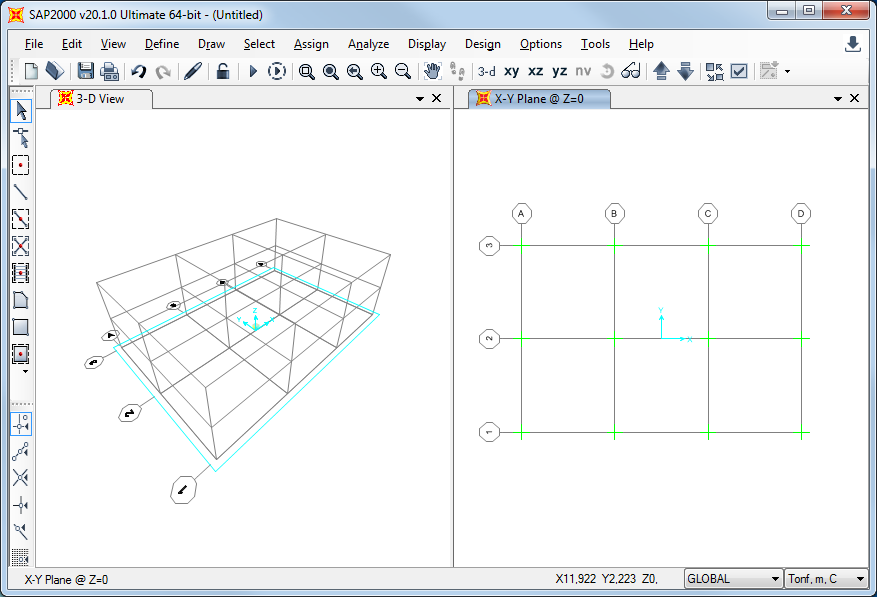
\includegraphics[width=1\textwidth]{metodologia/sap2000_axes.png}
%     \caption{Entorno virtual de SAP2000\textsuperscript{\textregistered} con un conjunto de ejes definido.}
%     \label{fig:sap2000_axes}
% \end{figure}

% Los menús del programa de computador que permiten ingresar los elementos del modelo consisten en aquellos que permiten escoger el tipo de elemento, como se muestra en la figura \ref{fig:sap200_draw}, y aquellos que permiten modificar los elementos ya ingresados, los cuales permiten moverlos, copiarlos, o eliminarlos. \\
% \begin{figure}[ht]
%     \centering
%     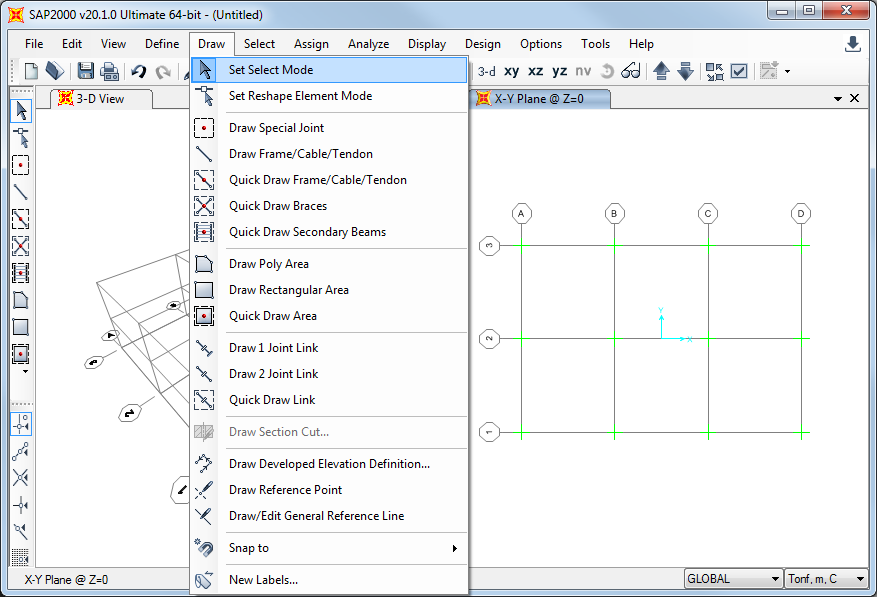
\includegraphics[width=1\textwidth]{metodologia/sap2000_draw.png}
%     \caption{Menú de SAP2000\textsuperscript{\textregistered} que permite ingresar diferentes tipos de elementos.}
%     \label{fig:sap200_draw}
% \end{figure}

% Una vez el usuario haya agregado los diferentes elementos de la estructura puede modificar sus condiciones de apoyo, las cargas, entre otros, mediante el uso de menús, de manera que el modelo esté listo para que el programa ejecute el análisis correspondiente. En la figura \ref{fig:sap2000_model} se presenta el modelo de una estructura terminado.
% \begin{figure}[ht]
%     \centering
%     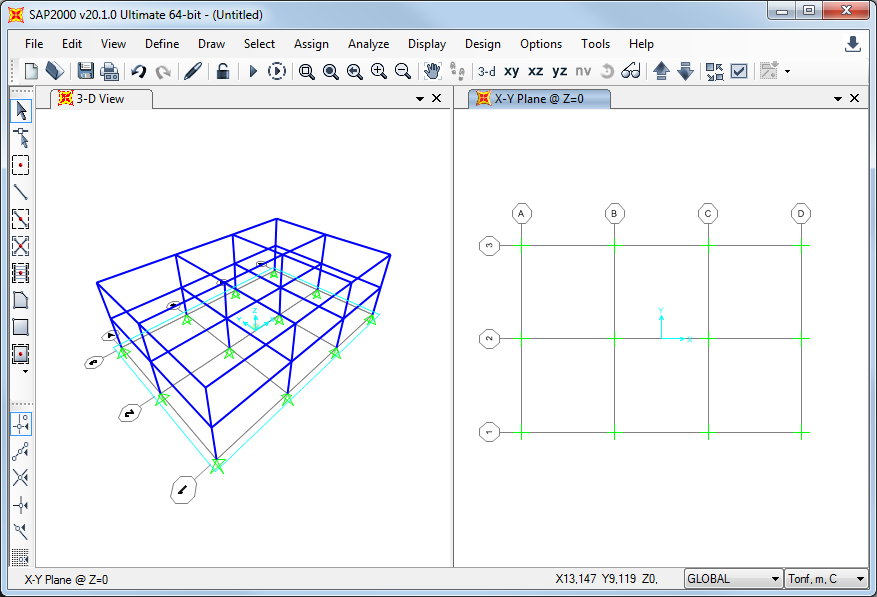
\includegraphics[width=1\textwidth]{metodologia/sap2000_model.png}
%     \caption{Modelo de una estructura en  SAP2000\textsuperscript{\textregistered}.}
%     \label{fig:sap2000_model}
% \end{figure}

% Una vez se han surtido los pasos anteriores, el usuario puede correr el análisis para obtener los resultados del mismo. El usuario puede visualizar los resultados en el entorno virtual, como se muestra en la figura \ref{fig:sap2000_deformed}, o mediante tablas.
% \begin{figure}[ht]
%     \centering
%     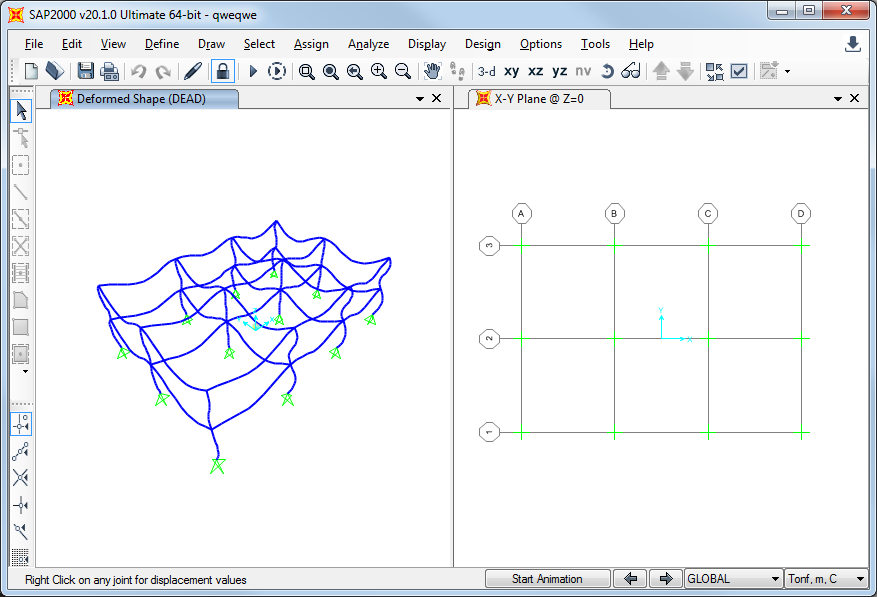
\includegraphics[width=1\textwidth]{metodologia/sap2000_deformed.png}
%     \caption{Deformación de la estructura después del análisis de SAP2000\textsuperscript{\textregistered}.}
%     \label{fig:sap2000_deformed}
% \end{figure}

% Así como el programa SAP2000\textsuperscript{\textregistered}, los otros programas comerciales, como ETABS \textsuperscript{\textregistered}, CSIBridge\textsuperscript{\textregistered}, midas\textsuperscript{\textregistered}, entre otros, cuentan con herramientas similares para que el usuario pueda analizar modelos de estructuras.

% \section{Revisión de los programas a código abierto}
% Existen gran variedad de programas a código abierto. Entre los programas que más se han estudiado para este trabajo se encuentra \textit{ANALEST}. \\

% El programa \textit{ANALEST} comprende una serie de subprogramas cuyo objeto es servir de ayuda en el análisis y diseño de estructuras. El programa está programado en \texttt{BASIC} y su característica principal es analizar 
% \begin{inparaenum}[$ (1) $]
%     \item vigas continúas, 
%     \item armaduras planas, 
%     \item armaduras en el espacio, 
%     \item pórticos planos, 
%     \item pórticos en el espacio, 
%     \item parrillas planas.
% \end{inparaenum}

% Para usar los subprogramas, se debe
% \begin{inparaenum}[$ (1) $]
%     \item introducir los datos del modelo de la estructura, revisarlos y guardarlos, 
%     \item introducir los datos de carga, revisarlos y guardarlos, 
%     \item ejecutar el análisis, guardar los resultados y presentarlos
% \end{inparaenum}

% Ademas, los subprogamas de vigas y armaduras permiten encontrar la envolvente de momentos en los apoyos y de fuerzas axiales, respectivamente, como paso preliminar para el diseño de los miembros. \\

% Guardar los datos estructurales y los datos de carga es muy útil en aquellos casos en que conviene modificar las dimensiones de los elementos con base en los resultados del primer análisis. Por otra parte, guardar los resultados facilita el estudio de las combinaciones de carga disminuyendo por una parte los datos requeridos y por otra el tiempo de ejecución, ya que se aprovecha el principio de superposición. Adicionalmente, guardar dichos resultados facilita el enlace de los subprogramas con programas de diseño, bien sean adquiridos o desarrollados por el usuario. \\

% \section{Identificación de los elementos a programar}

% De la revisión de los diferentes programas comerciales se dedujo que el programa StressUN debía dividirse en tres partes y que tenían que trabajar en conjunto. Dichas partes son: \textit{preproceso}, \textit{proceso} y \textit{posproceso}. \\

% El preproceso consiste en la adquisición de todos los datos relevantes del modelo de la estructura a analizar. El proceso realiza el tratamiento de los datos del modelo, mientras que el posproceso presenta los resultados del análisis del modelo. \\

% Tanto el preproceso como el posproceso necesitan de un ambiente gráfico, mientras que el proceso necesita de las rutinas propias del análisis matricial. \\

% \section{Selección de las herramientas de programación}
% Los dos grandes problemas a solucionar consistieron en desarrollar el ambiente gráfico, el cual se compone de menús y un entorno virtual tridimensional, y el núcleo de StressUN. Para esto, se consultó las diferentes herramientas de programación disponibles, donde se decidió utilizar la librería \textit{frames}, la cual está programada en el \textit{Java}, y el conjuto de librerías \textit{Scipy}, la cual está programada en \textit{Python}.\\

% La librería frames consiste en un conjunto de herramientas para crear un entorno virtual bidimensional o tridimensional interactivo. Dicha librería trabaja como una extensión de la librería \textit{processing}, la cual también está programada en Java. \\

% La librería processing es un conjunto de herramientas dirigida a solucionar los problemas relacionados con la computación gráfica, permitiendo a los desarrolladores desde crear imágenes hasta entornos virtuales tridimensionales. \\

% Por otro lado, el conjunto de librerías Scipy consiste en herramientas para solucionar problemas relacionados algebra matricial. Dicho conjunto de librerías está conformado por \textit{Numpy}, \textit{Scipy}, \textit{matplotlib}, entre otros. La librería Numpy provee arreglos multidimensionales y operaciones entre ellos. La librería \textit{Scipy} trata problemas del algebra matricial, como son la solución de sistemas de ecuaciones líneales, mientras que matplotlib permite generar diferentes tipos de gráficos. \\

% \section{Desarrollo del programa de computador}

% Una vez se identificaron los diferentes elementos necesarios con los que debía contar el programa de computador y se escogieron las herramientas de trabajo, se realizó una revisión bibliográfica de la formulación matemática de los métodos matriciales aplicados al análisis estructural, enfocada al análisis de estructuras tridimensionales de respuesta lineal. Adicionalmente, se realizó una revisión a la documentación de la librería frames.\\

% De dicho ejercicio se identificaron los datos de entrada que el usuario necesita definir y los datos de salida que espera obtener
% \begin{itemize}
%     \item \textit{Preproceso}
%     \begin{itemize}
%         \item Definición de los materiales.
%         \item Definición de las secciones transversales.
%         \item Definición de los nudos.
%         \item Definición de los elementos.
%         \item Definición de las condiciones de apoyo.
%         \item Definición de los casos de carga.
%         \item Definición de las combinaciones de carga.
%         \item Definición de las patrones de carga
%     \end{itemize}
%     \item \textit{Posproceso}
%     \begin{itemize}
%         \item Visualización de los desplazamientos en los nudos.
%         \item Visualización de las reacciones.
%         \item Visualización de las fuerzas internas.
%     \end{itemize}
    
% \end{itemize}

%  \textit{StressUN} se desarrolló usando el paradigma de \textit{programación orientada a objetos}, \textit{OOP} (de sus siglas en inglés \textit{object-oriented programming}), y en forma modular, de manera que el \textit{preproceso} y el \textit{posproceso} son independientes del \textit{proceso}.\\

% A medida que se definieron los diferentes elementos a tener en cuenta, se fueron programando. Es decir, se desarrollaron las clases \textit{primitivas} del programa, las cuales representan la abstracción de los elementos de las entidades más sencillas del problema, las cuales consisten en las clases
% \begin{itemize}
%     \item \textit{Material}.
%     \item \textit{Section}.
%     \item \textit{Node}.
%     \item \textit{Frame}.
%     \item \textit{Support}.
%     \item \textit{PointLoad}.
%     \item \textit{LoadPattern}.
%     \item \textit{Displacement}.
% \end{itemize}

% Las clases anteriormente listadas, tienen su representación tanto en el preproceso y posproceso, como en el proceso. Es decir, en el preproceso y posproceso dichas clases tienen su representación gráfica, mientras que en el proceso, éstos tienen su representación matemática. Sin embargo, dichas clases son separadas unas de las otras, de manera que se asegure que el preproceso y posproceso son independientes del proceso.

% Una vez programados las entidades más básicas del programa, se procedió a crear la clase \textit{Structure}, la cual se encarga de administrar otros objetos. Dicho paradigma de programación se conoce como \textit{composición}. Los objetos que contiene la clase \textit{Structure} son

% \begin{itemize}
%     \item \textit{Materials}.
%     \item \textit{Sections}.
%     \item \textit{Nodes}.
%     \item \textit{Frames}.
%     \item \textit{Supports}.
%     \item \textit{LoadPatterns}.
% \end{itemize}

% Cada una de las anteriores clases es la interfaz entre el programa y el usuario, donde este último podrá agregar nuevos materiales, secciones, nudos, elementos tipo pórtico, condiciones de apoyo y condiciones de carga. Dichas clases componen el \textit{núcleo} del programa.\\

% El proceso anteriormente descrito se desarrolló bajo los diferentes mecanismos que provee la programación orientada objeto, los cuales son encapsulación, herencia y sobre carga. Estas herramientas, bien aplicadas, permiten la reutilización del código y el mantenimiento del mismo. Así mismo, se utilizó la herramienta de \textit{Git}, la cual es un sistema de control de versiones, la cual permite llevar el control absoluto durante el proceso de desarrollo del código.\\

% \section{Verificación del programa}

% Una vez se llegó a una versión estable del programa, este se puso a prueba mediante la solución de diferentes problemas que aparecen en la bibliografía, donde se comparó la respuesta obtenida con la presentada. Así mismo, se comparó el desempeño del programa frente a otros programas, tanto comerciales como académicos, en cuanto a la facilidad de uso como al tiempo de computo. \\
% \chapter{pyFEM}
\label{cha:pyFEM}

En la figura \ref{fig:space-frame} se presenta un elemento \emph{i} tipo \emph{pórtico} con sus nodos \emph{j} y \emph{k} empotrados. El sistema de coordenadas locales del elemento tiene como origen el nodo \emph{j}. El eje $ x $ coincide con el eje centroidal del elemento y es positivo en el sentido del nodo \emph{j} al nodo \emph{k}. Los ejes $ y $ y $ z $ son los ejes principales del elemento de manera que los planos $ xy $ y $ zx $ son los planos principales de flexión. Se asume que el centro de cortante y el centroide del elemento coinciden de tal forma que la flexión y la torsión se presentan una independiente de la otra. Los grados de libertad se numeran del 1 al 12, empezando por las translaciones y las rotaciones del nodo \emph{j}, tomados en orden $ x $, $ y $, $ z $ respectivamente.

\begin{figure}[ht]
  \centering
  \begin{tikzpicture}[coords]
    % points
    \dpoint{a}{0}{0}{0};
    \dpoint{b}{4}{0}{0};

    \dpoint{alabel}{0}{0}{0.25};
    \dpoint{blabel}{4}{0}{0.25};

    \dpoint{beamlabel}{2}{0}{0.25};

    \dpoint{jux}{-1}{0}{0};
    \dpoint{juy}{0}{-1.5}{0.25};   
    \dpoint{juz}{0}{0}{-1.25};

    \dpoint{jrx}{-2}{0}{0};
    \dpoint{jry}{0}{-2.75}{0.25};   
    \dpoint{jrz}{0}{0}{-2.5};

    \dpoint{kux}{4.5}{0}{0};
    \dpoint{kuy}{4}{-1.5}{0.25};   
    \dpoint{kuz}{4}{0}{-1.25};

    \dpoint{krx}{5.25}{0}{0};
    \dpoint{kry}{4}{-2.75}{0.35};   
    \dpoint{krz}{4}{0}{-2.5};   
   
    % beams
    \dbeam{1}{a}{b};

    \dnotation{6}{beamlabel}{\emph{i}};

    % supports
    \dsupport{2}{a}[yz];
    \dsupport{2}{b}[yz];

    \dnotation{1}{alabel}{\emph{j}};
    \dnotation{1}{blabel}{\emph{k}};
    % restrains
    % j
    \dload{1}{a}[270][0][1];
    \dload{1}{a}[270][90][1][0.5];   
    \dload{1}{a}[180][180][1][0.5];

    \dload{3}{a}[270][0][1][1.25];
    \dload{3}{a}[270][90][1][1.75];   
    \dload{3}{a}[180][180][1][1.75];

    \dnotation{1}{jux}{1};
    \dnotation{1}{juy}{2};
    \dnotation{1}{juz}{3};

    \dnotation{1}{jrx}{4};
    \dnotation{1}{jry}{5};
    \dnotation{1}{jrz}{6};   
    
    % k
    \dload{2}{b}[90][0][1];
    \dload{1}{b}[270][90][1][0.5];   
    \dload{1}{b}[180][180][1][0.5];

    \dload{4}{b}[90][0][1][1.25];
    \dload{3}{b}[270][90][1][1.75];   
    \dload{3}{b}[180][180][1][1.75];

    \dnotation{1}{kux}{7};
    \dnotation{1}{kuy}{8};
    \dnotation{1}{kuz}{9};

    \dnotation{1}{krx}{10};
    \dnotation{1}{kry}{11};
    \dnotation{1}{krz}{12};
    
    % axes
    \dscaling{3}{1};
    \daxis{1}{0, 0, 0};
  \end{tikzpicture}
  \caption{Elemento tipo pórtico en coordenadas locales.}
  \label{fig:space-frame}
\end{figure}

Según \cite{weaver1990matrixanalysis}, (\ref{eq:matriz-rigidez-elemento-portico}) es la matrix de rigidez del elemento tipo pórtico en coordenadas locales, donde $ E $ es el módulo de elasticidad del material, $ G $ es el módulo de elasticidad a cortante del material, $ L $ es la longitud del elemento y $ A_x $, $ I_x $, $ I_y $ y $ I_z $ son el área, la constante de torsión y los momentos principales de inercia con respecto a los ejes $ y $ y $ z $ de la sección transversal.\\

\begin{equation}
  \begin{bNiceArray}{CCCCCCCCCCCC}[small,
    first-row,
    first-col,
    code-for-first-row = \mathbf{\arabic{jCol}},
    code-for-first-col = \mathbf{\arabic{iRow}}
    ]
    & & & & & & & & & & & & \\
    & \frac{EA_x}{L} & 0 & 0 & 0 & 0 & 0 & -\frac{EA_x}{L} & 0 & 0 & 0 & 0 & 0 \\
    & & \frac{12EI_z}{L^3} & 0 & 0 & 0 & \frac{6EI_z}{L^2} & 0 & -\frac{12EI_z}{L^3} & 0 & 0 & 0 & \frac{6EI_z}{L^2} \\
    & & & \frac{12EI_y}{L^3} & 0 & -\frac{6EI_y}{L^2} & 0 & 0 & 0 & -\frac{12EI_y}{L^3} & 0 & -\frac{6EI_y}{L^2} & 0 \\
    & & & & \frac{GI_x}{L} & 0 & 0 & 0 & 0 & 0 & -\frac{GI_x}{L} & 0 & 0 \\
    & & & & & \frac{4EI_y}{L} & 0 & 0 & 0 & \frac{6EI_y}{L^2} & 0 & \frac{2EI_y}{L} & 0 \\
    & & & & & & \frac{4EI_z}{L} & 0 & -\frac{6EI_z}{L^2} & 0 & 0 & 0 & \frac{2EI_z}{L} \\
    & & & & & & & \frac{EA_x}{L} & 0 & 0 & 0 & 0 & 0 \\
    & & & & & & & & \frac{12EI_z}{L^3} & 0 & 0 & 0 & -\frac{6EI_z}{L^2} \\
    & & & & & & & & & \frac{12EI_y}{L^3} & 0 & \frac{6EI_y}{L^2} & 0 \\
    & & & & & & & & & & \frac{GI_x}{L} & 0 & 0 \\
    & & & & & & & & & & & \frac{4EI_y}{L} & 0 \\
    & \emph{sim.} & & & & & & & & & & & \frac{4EI_z}{L}
    \label{eq:matriz-rigidez-elemento-portico}
  \end{bNiceArray}
\end{equation}  

Según \cite{dunn20023d}, la orientación en tres dimensiones se puede describir usando \emph{cuaterniones} que se definen como
\begin{equation}
  q = w + x\mathbf{i} + y\mathbf{j} + z\mathbf{k}
\end{equation}

Los cuaterniones extienden el sistema de números complejos al tener tres números imaginarios los cuales se relacionan de la siguiente manera
\begin{gather}
  i^2 = j^2 = k^2 = -1 \\
  ij = k, ji = -k \nonumber \\
  jk = i, kj = -i \nonumber \\
  ki = j, ik = -j \nonumber
\end{gather}
% \chapter{Metodología}
\label{chap:metodologia}
En el capítulo anterior se estudiaron las características de diversos programas de computador de análisis matricial, tanto académicos como comerciales, con el fin de
\begin{inparaenum}[$ (a) $]
    \item identificar los elementos que tienen en común y
    \item las ventajas y las desventajas que hay entre estos. \\
\end{inparaenum}

Con base en dicho estudio, el problema que debía solucionar el programa de computador a desarrollar, el cual consiste en resolver modelos de estructuras reticulares tridimensionales sometidas a cargas estáticas, y sus posibles características, se concluyó que el programa de computador debía contar con:

\begin{itemize}
    \item un procesador que analice la información del modelo de la estructura y la resuelva, siendo las rutinas empleadas accesibles a cualquier usuario
    
    \item un ambiente virtual tridimensional en el cual se pueda ingresar la información del modelo, se presente dicha información y la solución del mismo, el cual sea del agrado del usuario
    
    \item rutinas a código abierto, de manera que se pudieran estudiar, modificar y ampliar
\end{itemize} 

Una vez se determinó cómo debía ser el programa de computador, se encontró la necesidad de contar con  ciertas herramientas para dotar al programa de computador con la capacidad de resolver el problema en cuestión y que tuviera las características deseadas. \\

Lo anterior fue el insumo para desarrollar un programa de computador llamado \textit{StressUN}, en honor al programa de computador \textit{STRESS} (\textit{STRuctural Engineering System Solver}), desarrollado por un grupo de ingenieros en cabeza del profesor Fenves en la década de los años sesenta en el \textit{MIT} (de sus siglas en inglés, \textit{Massachusetts Institute of Technology}) \cite{fenves1965referenceUser}, dado que este trabajo comparte muchos de los criterios con los que el profesor concibió su programa. \\

A continuación se presenta la filosofía con la cual fue desarrollado el programa \textit{StressUN}, las herramientas empleadas para dicho desarrollo, se discute el porqué de dicha selección, los diferentes elementos que componen al programa y como funcionan.

\section{Filosofía de \textit{StressUN}}

El programa de computador \textit{StressUN} se concibió como una herramienta para solucionar modelos de estructuras reticulares tridimensionales sometidas a cargas estáticas que combinara las características de los programas tanto académicos como comerciales, para convertirse en una opción llamativa en las universidades. \\

Para lograr este objetivo, el programa \textit{StressUN} se caracteriza por ser práctico, es decir, en él se puede describir el modelo de la estructura y obtener los resultados de la solución de forma fácil e intuitiva y, por otro lado, se puede conocer cada una de las rutinas empleadas. \\

En dirección paralela a solucionar dichos modelos, se busca que \textit{StressUN}, en un futuro, se convierta en una opción para diseñadores e investigadores en su quehacer, el cual sea competitivo frente a programas comerciales, para lo cual, se analizó minuciosamente cada una de las herramientas disponibles que permitieran lograr tal objetivo ulterior. \\

De manera que no basta que solucione modelos de estructuras tridimensionales reticulares sometidas a cargas estáticas, ni que cuente con un ambiente virtual tridimensional donde se pueda ver la información del modelo de la estructura de forma interactiva, si no que se tenga acceso a sus rutinas, se les pueda modificar y agregar otras nuevas. \\

Para cumplir con las expectativas, se eligieron varias herramientas que se encuentran a la vanguardia y se implementarion en el programa de computador \textit{StressUN}, de tal manera que las rutinas de éste fueran fácilmente entendibles, modificables y ampliable.

\section{Componentes de \textit{StressUN}}

El programa de computador \textit{StressUN} está constituido por un \textit{pre} y \textit{pos procesador}, llamado \textit{StressUN}, y un conjunto de rutinas de programación llamado \textit{pyFEM}. El pre y posprocesador \textit{StressUN} consiste en un ambiente virtual tridimensional interactivo, el cual permite el ingreso de la información del modelo de la estructura, la visualización de dicha información y de los resultados de la solución, mientras las rutinas de programación \textit{pyFEM} provee las herramientas para encontrar la solución del modelo. \\

Para desarrollar cada uno de estos componentes, se uso el lenguaje de programación \textit{python} \cite{Rossum}, el ecosistema para ingeniería \textit{SciPy} \cite{Enthought} y el entorno de trabajo para visualizaciones tridimensionales \textit{Panda3D} \cite{TheWaltDisneyCompany}. \\

\subsection{Lenguaje de programación \textit{python}}

Se escogió el lenguaje de programación \textit{python} sobre los demás lenguajes presentados en el capítulo \textit{Antecedentes} porque
\begin{itemize}
    \item es fácil de aprender, lo que permite que se escriban instrucciones deseadas en un menor tiempo en comparación con otros lenguajes,
    \item la sintaxis hace que sea fácil de leer, de manera que el lector entenderá más rápido rutinas ya escritas,
    \item es interpretado, haciendo que el tiempo de desarrollo de rutinas sea menor al evitar el proceso de compilación para evidenciar errores en \textit{tiempo de ejecución}. Adicionalmente, al ser interpretado, se hace necesario tener todas las rutinas que se van a ejecutar (en lugar de un archivo compilado), de manera que pueden ser revisadas en cualquier momento,
    \item es multiproposito, por tanto se puede usar en aplicaciones de ingenieria hasta \textit{aplicaciones web}, pasando por administración de bases de datos, interfaces gráficas de usuario, aprendizaje de máquina, entre muchas otras,
    \item es multiplataforma, así que las mismas rutinas se pueden ejecutar en los principales sistemas operativos (\textit{Windows}, \textit{macOS} y las diferentes distribuciones de \textit{Linux}). Adicionalmente, las interfaces gráficas son \textit{nativas} en cada uno de los diferentes sistemas operativos,
    \item soporta, entre otros, el paradigma de programación orientada a objetos, lo cual permite evitar la redundancia de código, gracias a la generación de múltiples instancias de una misma clase y a la personalización de éstas vía herencia. También permite que los objetos tengan un comportamiento similar a los \textit{objetos primitivos} mediante la \textit{sobrecarga de operadores},
    \item es gratuito y a código abierto, en consecuencia no hay que pagar para usarlo, los programas desarrollados con él no están limitados por licencias y cuenta con una comunidad bastante activa presta a resolver las dudas que se presenten.
\end{itemize}

Sin embargo, una desventaja que presenta este lenguaje de programación es que toma más tiempo para ejecutar las mismas instrucciones que otros lenguaje de programación, como \textit{C++} o \textit{Java}. No obstante, existen implementaciones de \textit{python} como \textit{CPython} que permiten ejecutar instrucciones de \textit{C++} desde \textit{python}, haciendo de tal desventaja pequeña, de manera que no es un criterio para dejar de usar este lenguaje.

\subsection{Pre y pos procesador \textit{StressUN}}

Para desarrollar el ambiente virtual tridimensional interactivo se debía hacer uso de una herramienta que proveyera una \textit{escena}, la cual permite posicionar objetos en un espacio tridimensional, representarlos en la pantalla del computador desde el punto de vista de un observador y poder interactuar con ellos a través del ratón del computador. \\

Se escogió la librería \textit{Panda3D} sobre las demás librerías presentadas en el capítulo \textit{Antecedentes} porque
\begin{itemize}
    \item se puede usar con \textit{python}, de manera que todas las rutinas del programa de computador se hacen en el mismo lenguaje de programación, 
    \item las rutinas que se ejecutan están escritas en \textit{C++}, donde \textit{python} es un \textit{wrapper}, lo que permite un optimo desempeño del programa de computador al ejecutar rutinas compiladas, 
    \item es multiplataforma, así que las mismas rutinas se pueden ejecutar en los principales sitemas operativos (\textit{Windows}, \textit{macOS} y las diferentes distribuciones de \textit{Linux}), 
    \item cuenta con una comunidad activa, así que se puede acudir a ella en caso de tener problmas al tratar de implementar alguna rutina, 
    \item es gratuito y a código abierto, en consecuencia no hay que pagar para para usarlo y, al igual que \textit{python}, los programadas desarrollados con ella se pueden comercializar
\end{itemize}

Sin embargo, una desventaja que presenta esta libreria es que la documentación no está completa, lo que conlleva a especular o ignorar el comportamiento de la misma.

\subsection{pyFEm}

Para desarrollar las rutinas de programación \textit{pyFEM} se debía hacer uso de una herramienta que proveyera \textit{operaciones matriciales}, las cuales permitan sumar, restar y multiplicar matrices. \\

Se escogió el ecosistema para matemáticas, ciencias e ingeniería \textit{sciPy}, el cual está compuesto, entre otras, por las librerías \textit{NumPy}, \textit{SciPy}, \textit{Matplotlib} y \textit{pandas}, las que proveen arreglos \textit{n-dimensionales}, rutinas de programación científica (integración numerica y optimización), gráficas bidimensionales y análisis de datos estructurados, respectivamente. \\

Se escogió dicho ecosistemas sobre las demás librerias presentadas en el capítulo \textit{Antecedentes} porque:
\begin{itemize}
    \item se puede usar con \textit{python}, de manera que todas las rutinas del programa de computador se hacen en el mismo lenguaje de programación, 
    \item es multiplataforma, así que las mismas rutinas se pueden ejecutar en los principales sistemas operativos (\textit{Windows}, \textit{macOS} y las diferentes distribuciones de \textit{Linux}), 
    \item cuenta con una comunidad bastante activa, así que se puede acudir a ella en caso de tener probemas al tratar de implementar alguna rutina, 
    \item se puede integrar con \textit{C++} y \textit{Fortran}, de manera que se puede usar rutinas escritas en estos lenguajes o implementar las propias para optimizar el tiempo de cálculo, 
\end{itemize}

Sin embargo, una desventaja que se presenta en esta librería es que toma más tiempo para ejecutar las mismas instrucciones que otras librerías en otros lenguajes de programación, como \textit{C++} o \textit{C}. No obstante, esta librería está bastante optimizada, tanto así que si se llega a presentar que el tiempo de ejecución es bastante grande, esto se presentaría en otros lenguajes.

\subsection{Integración entre \textit{python} y las librerías}

En las secciones anteriores se presentaron las herramientas que fueron usadas para desarrollar el programa de computador \textit{StressUN}. A modo de resumen, dichas herramientas consisten en el lenguaje de programación \textit{python}, la liberría \textit{Panda3D} y el ecosistema \textit{sciPy}. \\

Estas herramientas cuentan con la gran ventaja que todas se pueden usar bajo el mismo lenguaje de programación, de manera que no hay necesidad de aprender más de un lenguaje de programación. \\

Así mismo, \textit{python} cuenta con la ventaje que, al ser interpretado, se deba tener las rutinas necesarias para ejecutar el programa, de manera tal que estas pueden ser leídas, estudiadas y modificadas en cualquier momento. \\

\subsection{Sistema de control de versiones}

Durante el desarrollo del programa de computador \textit{StressUN} se evidenció la necesidad de llevar el control de cada una de las nuevas rutinas implementadas, para lo cual se optó por usar el sistema de versión de controles \textit{GitHub}. \\

\textit{Github} permite guardar estados en el desarrollo del código, de manera que se puede experimentar con rutinas de programación y, una vez sean existosas, crear un punto de control al cual se puede regresar en cualquier momento.

\subsection{Classtools}

\begin{codigoprog}
class AttrDisplay:
    def gather_attrs(self):
    def __repr__(self):
\end{codigoprog}

\begin{codigoprog}
class Collection:
    def __init__(self):
    def add(self, obj):
    def _labels(self):
    def __getitem__(self, item):
    def __iter__(self):
    def __len__(self):
    def __repr__(self):
\end{codigoprog}

\subsection{Primitives}

\begin{codigoprog}
class Material(AttrDisplay):
    def __init__(self, label, modulus_elasticity, modulus_elasticity_shear):
    def __eq__(self, other):
\end{codigoprog}

\begin{codigoprog}
class Section(AttrDisplay):
    def __init__(self, label, material, area, moment_inertia_y, moment_inertia_z, torsion_constant):
    def __eq__(self, other):
\end{codigoprog}

\begin{codigoprog}
class Node(AttrDisplay):
    def __init__(self, label, x, y, z):
    def set_degrees_freedom(self, u):
    def __eq__(self, other):
\end{codigoprog}

\begin{codigoprog}
class Truss(AttrDisplay):
    number_dimensions = 3
    number_nodes = 2
    number_degrees_freedom_per_node = 3

    def __init__(self, label, node_i, node_j, section):
    def get_local_vector(self):
    def get_orientation(self):
    def get_matrix_transformation(self):
    def get_local_stiff_matrix(self):
    def get_global_stiff_matrix(self):
    def get_modulus(self):
    def get_area(self):
    def get_length(self):
    def get_forces(self, load_pattern):
    def __eq__(self, other):
\end{codigoprog}

\begin{codigoprog}
class Frame(Truss):
    number_degrees_freedom_per_node = 6
    
    def get_local_stiff_matrix(self):
\end{codigoprog}

\begin{codigoprog}
class Support(AttrDisplay):
    def __init__(self, node, ux, uy, uz, rx, ry, rz):
    def __eq__(self, other):
\end{codigoprog}

\begin{codigoprog}
class PointLoad(AttrDisplay):
    def __init__(self, node, fx, fy, fz):
    def __eq__(self, other):
\end{codigoprog}

\begin{codigoprog}
class DistributedLoad(AttrDisplay):
    def __init__(self, frame, fx, fy, fz):
    def __eq__(self, other):
        return self.frame == other.frame
\end{codigoprog}

\begin{codigoprog}
class Displacement(AttrDisplay):
    def __init__(self, load_pattern, ux, uy, uz, rx, ry, rz):
\end{codigoprog}

\begin{codigoprog}
class Reaction(AttrDisplay):
    def __init__(self, load_pattern, reactions):
\end{codigoprog}

\begin{codigoprog}
class LoadPattern(AttrDisplay):
    def __init__(self, label, parent):
    def get_f(self):
    def __eq__(self, other):
\end{codigoprog}

\begin{codigoprog}
class PointLoads(Collection):
    def __init__(self, parent):
    def add(self, node, fx, fy, fz):
\end{codigoprog}

\begin{codigoprog}
class DistributedLoads(Collection):
    def __init__(self, parent):
    def add(self, frame, fx, fy, fz):
\end{codigoprog}

\begin{codigoprog}
class Displacements(Collection):
    def __init__(self):
    def add(self, load_pattern, ux, uy, uz, rx, ry, rz):
\end{codigoprog}

\begin{codigoprog}
class Reactions(Collection):
    def __init__(self):
    def add(self, load_pattern, reactions):
\end{codigoprog}


 \subsection{core}
 
\begin{codigoprog}
class Materials(Collection):
    def __init__(self, parent):
    def add(self, label, modulus_elasticity, modulus_elasticity_shear):
\end{codigoprog}

\begin{codigoprog}
class Sections(Collection):
    def __init__(self, parent):
    def add(self, label, material, area, inertia_y, inertia_z, torsion_constant):
\end{codigoprog}

\begin{codigoprog}
class Nodes(Collection):
    def __init__(self, parent):
    def add(self, label, x, y, z):
\end{codigoprog}

\begin{codigoprog}
class Trusses(Collection):
    def __init__(self, parent):
    def add(self, label, node_i, node_j, section):
\end{codigoprog}

\begin{codigoprog}
class Frames(Trusses):
    def __init__(self, parent):
    def add(self, label, node_i, node_j, section):
\end{codigoprog}

\begin{codigoprog}
class Supports(Collection):
    def __init__(self, parent):
    def add(self, node, ux, uy, uz, rx, ry, rz):
\end{codigoprog}

\begin{codigoprog}
class LoadPatterns(Collection):
    def __init__(self, parent):
    def add(self, label):
\end{codigoprog}

\begin{codigoprog}
class Structure:
    number_degrees_freedom_per_node = 6
    number_dimensions = 3

    def __init__(self):
    def set_degrees_freedom(self):
    def get_k(self):
    def solve(self):
    def __repr__(self):
\end{codigoprog}



% \section{StressUN}


% Los programas de computador comerciales para el análisis de estructuras mediante el método matricial que se encuentran vigentes cuentan, en general, con un entorno gráfico que le permite al usuario introducir los datos del modelo de forma interactiva, corregirlos, procesarlos y visualizar los resultados. \\

% Dado que la intención de este trabajo es desarrollar un programa de computador a código abierto que cuente con características similares a los programas comerciales, en este capítulo se inicia identificando dichas características. Así mismo, se estudian las características de los programas a código abierto. \\

% \section{Revisión de los programas comerciales}
% La intensión de este trabajo fue realizar un programa de computador llamado \textit{StressUN} similar a los programas comerciales, de tal manera que se procedió a estudiar los diferentes elementos que los caracterizan. \\

% Por ejemplo, SAP2000\textsuperscript{\textregistered} es un de estos programas de computador, ampliamente conocido en el ámbito colombiano. Para usarlo, el usuario primeramente debe definir las características de la estructura mediante una serie de menús, como se muestra en la figura \ref{fig:sap2000_toolbar}. El programa permite establecer tipos de materiales, secciones transversales de los elementos, patrones de carga, entre otras características.

% \begin{figure}[ht]
%     \centering
%     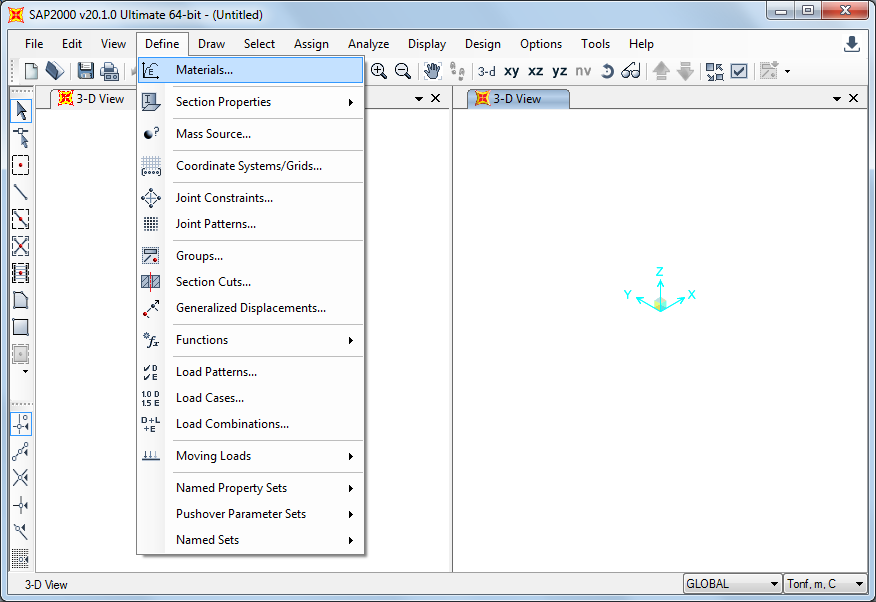
\includegraphics[width=1\textwidth]{metodologia/sap2000_toolbar.png}
%     \caption{Menús del programa de computador SAP2000\textsuperscript{\textregistered} para definir las características de la estructura.}
%     \label{fig:sap2000_toolbar}
% \end{figure}

% Una vez definidas las características de la estructura, el usuario procede a ingresar los diferentes elementos del modelo de la estructura en el entorno virtual de manera interactiva, mediante la ayuda de una serie de ejes y de los menús del programa. \\

% El entorno virtual consiste en un ambiente tridimensional donde el usuario puede ver, ingresar e interactuar con los diferentes elementos visuales del modelo.\\

% La serie de ejes consiste en un grupo de líneas en el espacio que se interceptan en un conjunto de puntos, los cuales sirven de referencia para que el usuario pueda ingresar los diferentes elementos del modelo al entorno virtual. En la figura \ref{fig:sap2000_axes} se presenta un conjunto de dichos ejes en el entorno virtual.\\
% \begin{figure}[ht]
%     \centering
%     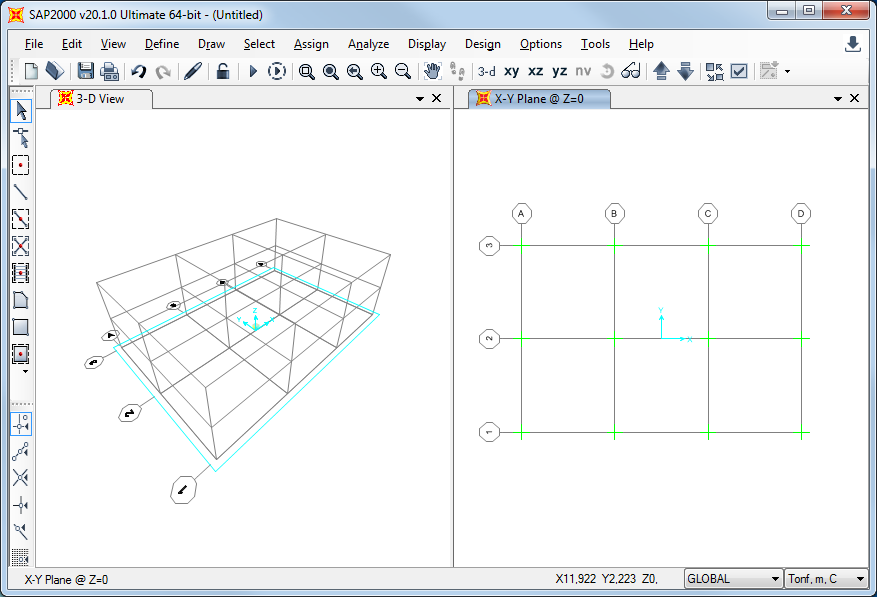
\includegraphics[width=1\textwidth]{metodologia/sap2000_axes.png}
%     \caption{Entorno virtual de SAP2000\textsuperscript{\textregistered} con un conjunto de ejes definido.}
%     \label{fig:sap2000_axes}
% \end{figure}

% Los menús del programa de computador que permiten ingresar los elementos del modelo consisten en aquellos que permiten escoger el tipo de elemento, como se muestra en la figura \ref{fig:sap200_draw}, y aquellos que permiten modificar los elementos ya ingresados, los cuales permiten moverlos, copiarlos, o eliminarlos. \\
% \begin{figure}[ht]
%     \centering
%     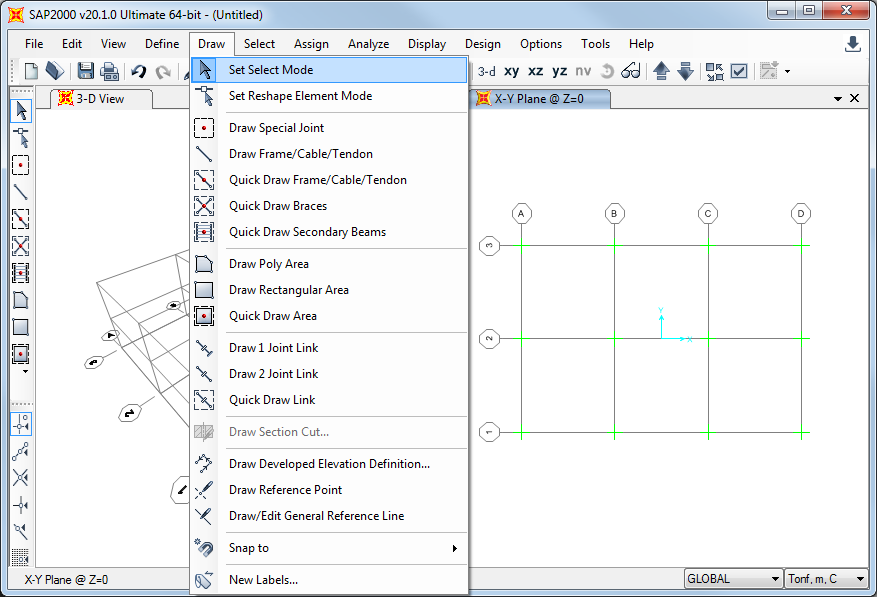
\includegraphics[width=1\textwidth]{metodologia/sap2000_draw.png}
%     \caption{Menú de SAP2000\textsuperscript{\textregistered} que permite ingresar diferentes tipos de elementos.}
%     \label{fig:sap200_draw}
% \end{figure}

% Una vez el usuario haya agregado los diferentes elementos de la estructura puede modificar sus condiciones de apoyo, las cargas, entre otros, mediante el uso de menús, de manera que el modelo esté listo para que el programa ejecute el análisis correspondiente. En la figura \ref{fig:sap2000_model} se presenta el modelo de una estructura terminado.
% \begin{figure}[ht]
%     \centering
%     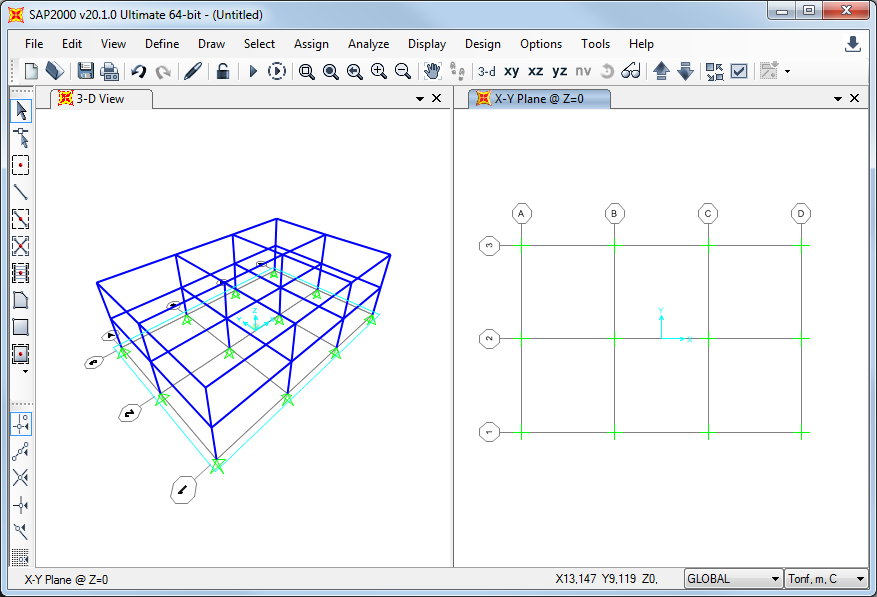
\includegraphics[width=1\textwidth]{metodologia/sap2000_model.png}
%     \caption{Modelo de una estructura en  SAP2000\textsuperscript{\textregistered}.}
%     \label{fig:sap2000_model}
% \end{figure}

% Una vez se han surtido los pasos anteriores, el usuario puede correr el análisis para obtener los resultados del mismo. El usuario puede visualizar los resultados en el entorno virtual, como se muestra en la figura \ref{fig:sap2000_deformed}, o mediante tablas.
% \begin{figure}[ht]
%     \centering
%     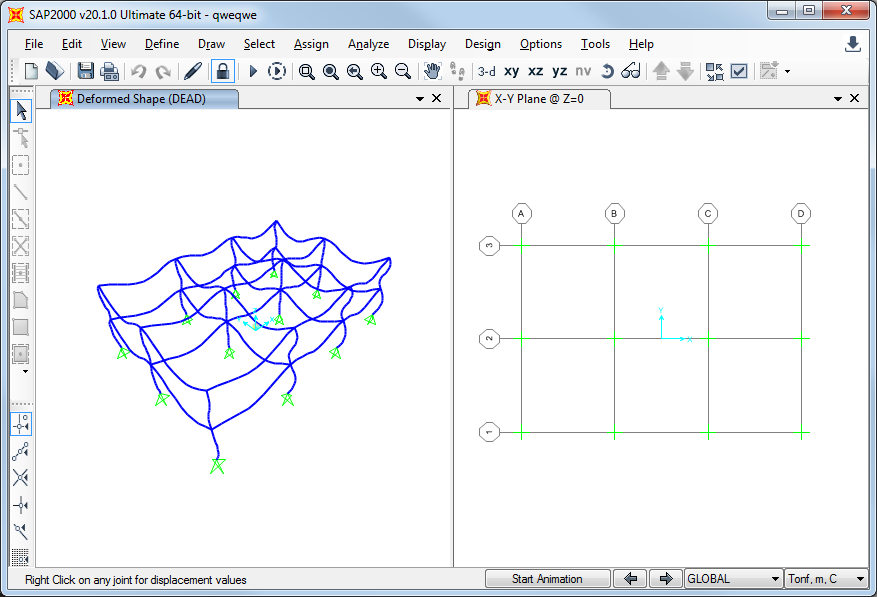
\includegraphics[width=1\textwidth]{metodologia/sap2000_deformed.png}
%     \caption{Deformación de la estructura después del análisis de SAP2000\textsuperscript{\textregistered}.}
%     \label{fig:sap2000_deformed}
% \end{figure}

% Así como el programa SAP2000\textsuperscript{\textregistered}, los otros programas comerciales, como ETABS \textsuperscript{\textregistered}, CSIBridge\textsuperscript{\textregistered}, midas\textsuperscript{\textregistered}, entre otros, cuentan con herramientas similares para que el usuario pueda analizar modelos de estructuras.

% \section{Revisión de los programas a código abierto}
% Existen gran variedad de programas a código abierto. Entre los programas que más se han estudiado para este trabajo se encuentra \textit{ANALEST}. \\

% El programa \textit{ANALEST} comprende una serie de subprogramas cuyo objeto es servir de ayuda en el análisis y diseño de estructuras. El programa está programado en \texttt{BASIC} y su característica principal es analizar 
% \begin{inparaenum}[$ (1) $]
%     \item vigas continúas, 
%     \item armaduras planas, 
%     \item armaduras en el espacio, 
%     \item pórticos planos, 
%     \item pórticos en el espacio, 
%     \item parrillas planas.
% \end{inparaenum}

% Para usar los subprogramas, se debe
% \begin{inparaenum}[$ (1) $]
%     \item introducir los datos del modelo de la estructura, revisarlos y guardarlos, 
%     \item introducir los datos de carga, revisarlos y guardarlos, 
%     \item ejecutar el análisis, guardar los resultados y presentarlos
% \end{inparaenum}

% Ademas, los subprogamas de vigas y armaduras permiten encontrar la envolvente de momentos en los apoyos y de fuerzas axiales, respectivamente, como paso preliminar para el diseño de los miembros. \\

% Guardar los datos estructurales y los datos de carga es muy útil en aquellos casos en que conviene modificar las dimensiones de los elementos con base en los resultados del primer análisis. Por otra parte, guardar los resultados facilita el estudio de las combinaciones de carga disminuyendo por una parte los datos requeridos y por otra el tiempo de ejecución, ya que se aprovecha el principio de superposición. Adicionalmente, guardar dichos resultados facilita el enlace de los subprogramas con programas de diseño, bien sean adquiridos o desarrollados por el usuario. \\

% \section{Identificación de los elementos a programar}

% De la revisión de los diferentes programas comerciales se dedujo que el programa StressUN debía dividirse en tres partes y que tenían que trabajar en conjunto. Dichas partes son: \textit{preproceso}, \textit{proceso} y \textit{posproceso}. \\

% El preproceso consiste en la adquisición de todos los datos relevantes del modelo de la estructura a analizar. El proceso realiza el tratamiento de los datos del modelo, mientras que el posproceso presenta los resultados del análisis del modelo. \\

% Tanto el preproceso como el posproceso necesitan de un ambiente gráfico, mientras que el proceso necesita de las rutinas propias del análisis matricial. \\

% \section{Selección de las herramientas de programación}
% Los dos grandes problemas a solucionar consistieron en desarrollar el ambiente gráfico, el cual se compone de menús y un entorno virtual tridimensional, y el núcleo de StressUN. Para esto, se consultó las diferentes herramientas de programación disponibles, donde se decidió utilizar la librería \textit{frames}, la cual está programada en el \textit{Java}, y el conjuto de librerías \textit{Scipy}, la cual está programada en \textit{Python}.\\

% La librería frames consiste en un conjunto de herramientas para crear un entorno virtual bidimensional o tridimensional interactivo. Dicha librería trabaja como una extensión de la librería \textit{processing}, la cual también está programada en Java. \\

% La librería processing es un conjunto de herramientas dirigida a solucionar los problemas relacionados con la computación gráfica, permitiendo a los desarrolladores desde crear imágenes hasta entornos virtuales tridimensionales. \\

% Por otro lado, el conjunto de librerías Scipy consiste en herramientas para solucionar problemas relacionados algebra matricial. Dicho conjunto de librerías está conformado por \textit{Numpy}, \textit{Scipy}, \textit{matplotlib}, entre otros. La librería Numpy provee arreglos multidimensionales y operaciones entre ellos. La librería \textit{Scipy} trata problemas del algebra matricial, como son la solución de sistemas de ecuaciones líneales, mientras que matplotlib permite generar diferentes tipos de gráficos. \\

% \section{Desarrollo del programa de computador}

% Una vez se identificaron los diferentes elementos necesarios con los que debía contar el programa de computador y se escogieron las herramientas de trabajo, se realizó una revisión bibliográfica de la formulación matemática de los métodos matriciales aplicados al análisis estructural, enfocada al análisis de estructuras tridimensionales de respuesta lineal. Adicionalmente, se realizó una revisión a la documentación de la librería frames.\\

% De dicho ejercicio se identificaron los datos de entrada que el usuario necesita definir y los datos de salida que espera obtener
% \begin{itemize}
%     \item \textit{Preproceso}
%     \begin{itemize}
%         \item Definición de los materiales.
%         \item Definición de las secciones transversales.
%         \item Definición de los nudos.
%         \item Definición de los elementos.
%         \item Definición de las condiciones de apoyo.
%         \item Definición de los casos de carga.
%         \item Definición de las combinaciones de carga.
%         \item Definición de las patrones de carga
%     \end{itemize}
%     \item \textit{Posproceso}
%     \begin{itemize}
%         \item Visualización de los desplazamientos en los nudos.
%         \item Visualización de las reacciones.
%         \item Visualización de las fuerzas internas.
%     \end{itemize}
    
% \end{itemize}

%  \textit{StressUN} se desarrolló usando el paradigma de \textit{programación orientada a objetos}, \textit{OOP} (de sus siglas en inglés \textit{object-oriented programming}), y en forma modular, de manera que el \textit{preproceso} y el \textit{posproceso} son independientes del \textit{proceso}.\\

% A medida que se definieron los diferentes elementos a tener en cuenta, se fueron programando. Es decir, se desarrollaron las clases \textit{primitivas} del programa, las cuales representan la abstracción de los elementos de las entidades más sencillas del problema, las cuales consisten en las clases
% \begin{itemize}
%     \item \textit{Material}.
%     \item \textit{Section}.
%     \item \textit{Node}.
%     \item \textit{Frame}.
%     \item \textit{Support}.
%     \item \textit{PointLoad}.
%     \item \textit{LoadPattern}.
%     \item \textit{Displacement}.
% \end{itemize}

% Las clases anteriormente listadas, tienen su representación tanto en el preproceso y posproceso, como en el proceso. Es decir, en el preproceso y posproceso dichas clases tienen su representación gráfica, mientras que en el proceso, éstos tienen su representación matemática. Sin embargo, dichas clases son separadas unas de las otras, de manera que se asegure que el preproceso y posproceso son independientes del proceso.

% Una vez programados las entidades más básicas del programa, se procedió a crear la clase \textit{Structure}, la cual se encarga de administrar otros objetos. Dicho paradigma de programación se conoce como \textit{composición}. Los objetos que contiene la clase \textit{Structure} son

% \begin{itemize}
%     \item \textit{Materials}.
%     \item \textit{Sections}.
%     \item \textit{Nodes}.
%     \item \textit{Frames}.
%     \item \textit{Supports}.
%     \item \textit{LoadPatterns}.
% \end{itemize}

% Cada una de las anteriores clases es la interfaz entre el programa y el usuario, donde este último podrá agregar nuevos materiales, secciones, nudos, elementos tipo pórtico, condiciones de apoyo y condiciones de carga. Dichas clases componen el \textit{núcleo} del programa.\\

% El proceso anteriormente descrito se desarrolló bajo los diferentes mecanismos que provee la programación orientada objeto, los cuales son encapsulación, herencia y sobre carga. Estas herramientas, bien aplicadas, permiten la reutilización del código y el mantenimiento del mismo. Así mismo, se utilizó la herramienta de \textit{Git}, la cual es un sistema de control de versiones, la cual permite llevar el control absoluto durante el proceso de desarrollo del código.\\

% \section{Verificación del programa}

% Una vez se llegó a una versión estable del programa, este se puso a prueba mediante la solución de diferentes problemas que aparecen en la bibliografía, donde se comparó la respuesta obtenida con la presentada. Así mismo, se comparó el desempeño del programa frente a otros programas, tanto comerciales como académicos, en cuanto a la facilidad de uso como al tiempo de computo. \\
% \chapter{Ejemplos de aplicación}
\label{chap:ejemplos_aplicacion}

Con el fin de presentar el funcionamiento de los programas desarrollados, en este capítulo se presentan diferentes modelos de estructuras tridimensionales de elementos rectos sometidos a cargas estáticas, los cuales se resuelven usando la librería \textit{pyFEM} o el programa de computador \textit{StressUN}. \\

\section{Funcionamiento de la librería \textit{pyFEM}} \label{sec:libreriaPyFem}
Se presentan varios ejemplos provenientes de los libros de la referencia bibliográfica, los cuales se resuelven usando el programa \textit{StressUN} o la librería \textit{pyFEM}, con el objetivo de comparar la respuesta obtenida con la presentada en dichos textos.

\subsection{Cercha plana}

En el libro \textit{Microcomputadores en Ingeniería Estructural}, del ingeniero \textit{Jairo Uribe Escamilla} (\cite{escamilla1995microcomputadores}), se presenta el ejemplo y la solución del modelo de una cercha simple plana estáticamente determinada (una cercha simple plana es una estructura compleja generada a partir de una estructura triangular base \cite{beer1997mecanica}). El ejercicio consiste en encontrar los desplazamientos de los nudos, las fuerzas de las reacciones y las fuerzas de cada elemento de la cercha mostrada en la figura \ref{fig:primer_punto}. La solución presenta las matrices de rigidez de cada uno de los elementos de la cercha, la matriz de rigidez de toda la estructura, la solución de los desplazamientos de los nodos, las reacciones de los apoyos y las fuerzas internas de cada elemento.\\

A continuación se presenta la solución de dicho ejemplo, el cual se resuelve usando la librería \texttt{pyFEM}. \\

\textit{\textbf{Ejemplo 7.1 -} Resuelva completamente la cercha mostrada por el método matricial de los desplazamientos. El material es acero estructural con $ E = 2040\; t / cm^2 $. Las áreas están dadas entre paréntesis en $ cm^2 $.}\\

\textit{\textbf{Solución -}} Para solucionar el ejemplo anterior usando la librería \texttt{pyFEM}, se ingresa la información necesaria para describir completamente el modelo de la estructura mediante instrucciones en el lenguaje de programación \texttt{python}, las cuales se almacenan en un archivo de texto plano. Dicha información consiste en:
\begin{inparaenum} [$ (1) $]
    \item los materiales,
    \item las secciones transversales,
    \item los nodos,
    \item los elementos tipo cercha,
    \item los apoyos y
    \item las cargas.
\end{inparaenum} \\

\begin{figure}[t]
    \centering
    
    \begin{tikzpicture}
        % Scaling
        % \scaling{.25};
        
        % Points
        \point{1}{0}{0};
        \point{2}{8}{0};
        \point{3}{4}{3};
        \point{4}{4}{0};
        
        \point{p}{4}{-1.3};
        \point{q}{5.05}{3.7875};
        
        \point{1-3}{2}{1.5};
        \point{1-4}{2}{0};
        \point{3-2}{6}{1.5};
        \point{4-2}{6}{0};
        \point{4-3}{4}{1.5};
        
        % Beams
        \beam{2}{1}{3}[0][0];
        \beam{2}{1}{4}[1][1];
        \beam{2}{3}{2}[1][1];
        \beam{2}{4}{2}[1][1];
        \beam{2}{4}{3}[1][1];
        
        % Supports
        \support{1}{1};
        \support{2}{2};
        
        % Joints
        \hinge{1}{1};
        \hinge{1}{2};
        \hinge{1}{3};
        \hinge{1}{4};
        
        % Loads
        \load{1}{q}[216.87];
        \load{1}{p}[90];
        
        % notation
        \notation{1}{1}{1}[above left];
        \notation{1}{2}{2}[above right];
        \notation{1}{3}{3}[above left];
        \notation{1}{4}{4}[below left];
        
        \notation{1}{3}{$ \SI{5}{\tonne} $}[above right=10mm];
        \notation{1}{4}{$ \SI{20}{\tonne} $}[below right=5mm and 0mm];
        
        \notation{5}{1}{3}[$ (100) $ ][.5][above][0.5];
        \notation{5}{1}{4}[$ (40) $ ][.5][above][0.5];
        \notation{5}{3}{2}[$ (150) $ ][.5][above][0.5];
        \notation{5}{4}{2}[$ (40) $ ][.5][above][0.5];
        \notation{5}{4}{3}[$ (30) $ ][.5][right][1];
        
        
        % Dimensions
        \dimensioning{1}{1}{4}{-1.5}[$ \SI{4}{m} $];
        \dimensioning{1}{4}{2}{-1.5}[$ \SI{4}{m} $];
        \dimensioning{2}{2}{3}{9}[$ \SI{3}{m} $];
    \end{tikzpicture}
    
    \caption{Cercha simple plana del \textit{Ejemplo 7.1} de \cite{escamilla1995microcomputadores}.}
    \label{fig:primer_punto}
\end{figure}

En el algoritmo \ref{alg:cercha_plana} se presentan las instrucciones que debe recibir \texttt{pyFEM} para solucionar el modelo de la estructura. Las instrucciones consisten en crear un nuevo objeto tipo \texttt{Structure}, al cual se le ha dado el nombre de \textit{structure} y, seguidamente, se agregan los materiales, las secciones, los nodos, los elementos tipo cercha, los apoyos, los patrones de carga y las cargas en los nodos. Una vez los datos del modelo de la estructura han sido ingresados, se puede solucionar el modelo mediante la instrucción \texttt{structure.solve()}. \\

\begin{lstlisting}[language=Python,caption=Ingreso de los datos del modelo de la estructura a \textit{pyFEM}.,label=alg:cercha_plana, frame=single]
# create structure
structure = Structure()

# add material
structure.materials.add("acero", 2040e4)

# add sections
structure.sections.add("section1", "acero", 30e-4)
structure.sections.add("section2", "acero", 40e-4)
structure.sections.add("section3", "acero", 100e-4)
structure.sections.add("section4", "acero", 150e-4)

# add nodes
structure.nodes.add('1', 0, 0, 0)
structure.nodes.add('2', 8, 0, 0)
structure.nodes.add('3', 4, 3, 0)
structure.nodes.add('4', 4, 0, 0)

# add trusses
structure.trusses.add('1-3', '1', '3', "section3")
structure.trusses.add('1-4', '1', '4', "section2")
structure.trusses.add('3-2', '3', '2', "section4")
structure.trusses.add('4-2', '4', '2', "section2")
structure.trusses.add('4-3', '4', '3', "section1")

# add support
structure.supports.add('1', True, True, True)
structure.supports.add('2', False, True, True)
structure.supports.add('3', False, False, True)
structure.supports.add('4', False, False, True)

# add load pattern
structure.load_patterns.add("point loads")

# add point loads
structure.load_patterns["point loads"].point_loads.add('4', 0, -20, 0)
structure.load_patterns["point loads"].point_loads.add('3', 5*0.8, 5*0.6, 0)

# solve the structure
structure().solve()
\end{lstlisting}

Cuando se ejecuta la instrucción \texttt{structure.solve()}, \texttt{pyFEM} comienza a solucionar el modelo de la estructura con base en la información ingresada. Los pasos que se efectúan para solucionar la estructura consisten en: 
\begin{inparaenum}[$ (1) $]
    \item asignar los grados de libertad de los nodos, 
    \item ensamblar la matriz de rigidez del modelo de la estructura, 
    \item imponer las condiciones de apoyo en la matriz de rigidez del modelo, 
    \item ensamblar el vector de fuerzas en los nodos para cada uno de los patrones de carga, 
    \item imponer las condiciones de apoyo en el vector de fuerzas en los nodos para cada caso de carga, 
    \item encontrar los desplazamientos de los nodos para cada patrón de carga, 
    \item encontrar las reacciones en los apoyos para cada patrón de carga y
    \item guardar la solución en los nodos y en los apoyos para cada patrón de carga.
\end{inparaenum} \\

A continuación se presenta el resultado de cada uno de los pasos realizados por \texttt{pyFEM} para solucionar la cercha del ejemplo 7.1. \\

\subsubsection{Grados de libertad de los nodos}
Para realizar el ensamblaje de la matriz de rigidez del modelo de la estructura y del vector de fuerzas de los nodos, se asignan números a los grados de libertad de los nodos de la estructura en el orden en que fueron ingresados. \\

Con base en ésto y en el algoritmo \ref{alg:cercha_plana}, el nodo \textit{'1'} se le han asignado los grados de libertad \textit{0, 1} y \textit{2}, al nodo \textit{'2'} los grados de libertad \textit{3, 4} y \textit{5}, y así sucesivamente.

\subsubsection{Matrices de rígidez}
Una vez se establecen los grados de libertad de los nodos del modelo de la estructura, se ensambla la matriz de rigidez del modelo de la estructura. Este proceso consiste en calcular una a una las matrices de rigidez de los elementos ensamblandolas en la matriz de rigidez del modelo, la cual, inicialmente, es una matriz de ceros. \\

Aunque no se almacenan las matrices de rigidez de cada uno de los elementos del modelo de la estructura, el usuario puede consultarlas. En la tabla \ref{tab:k_1_3} se presenta la matriz de rigidez en coordenadas globales del elemento \textit{1-3}, con sus respectivos grados de libertad, la cual se obtiene mediante la instrucción \textit{\textit{structure.trusses['1-3'].get\_global\_stiff\_matrix()}}. \\

\begin{table}[ht]
    \centering
    \begin{blockarray}{ccccccc}
        & \textit{0} & \textit{1} & \textit{2} & \textit{6} & \textit{7} & \textit{8} \\
        \begin{block}{c[cccccc]}
            \textit{0} & 26112 & 19584 & 0 & -261112 & -19584 & 0 \\
            \textit{1} & 19584 & 14688 & 0 & -19584 & -14688 & 0 \\
            \textit{2} & 0 & 0 & 0 & 0 & 0 & 0 \\
            \textit{3} & -26112 & -19584 & 0 & 26112 & 19584 & 0 \\
            \textit{4} & -19584 & -14688 & 0 & 19584 & 14688 & 0 \\
            \textit{5} & 0 & 0 & 0 & 0 & 0 & 0 \\
        \end{block}
    \end{blockarray} \si[per-mode=symbol]{\tonne\per\meter}
    \caption{Matriz de rigidez en coordenadas globales del elemento \textit{1-3}.}
    \label{tab:k_1_3}
\end{table}

En las tablas \ref{tab:k_1_4} a la \ref{tab:k_4_3} se presentan las matrices de rigidez en coordenadas globales de los demás elementos de la estructura, las cuales se obtienen con instrucciones similares a la anterior. \\

\begin{table}[h]
    \centering
    \begin{blockarray}{ccccccc}
        & \textit{0} & \textit{1} & \textit{2} & \textit{9} & \textit{10} & \textit{11} \\
        \begin{block}{c[cccccc]}
            \textit{0} & 20400 & 0 & 0 & -20400 & 0 & 0 \\
            \textit{1} & 0 & 0 & 0 & 0 & 0 & 0 \\
            \textit{2} & 0 & 0 & 0 & 0 & 0 & 0 \\
            \textit{9} & -20400 & 0 & 0 & 20400 & 0 & 0 \\
            \textit{10} & 0 & 0 & 0 & 0 & 0 & 0 \\
            \textit{11} & 0 & 0 & 0 & 0 & 0 & 0 \\
        \end{block} 
    \end{blockarray} \si[per-mode=symbol]{\tonne\per\meter}
    \caption{Matriz de rigidez en coordenadas globales del elemento \textit{1-4}.}
    \label{tab:k_1_4}
\end{table}

\begin{table}[ht]
    \centering
    \begin{blockarray}{ccccccc}
        & \textit{6} & \textit{7} & \textit{8} & \textit{3} & \textit{4} & \textit{5} \\
        \begin{block}{c[cccccc]}
            \textit{6} & 39168 & -29376 & 0 & -39168 & 29376 & 0 \\
            \textit{7} & -29376 & 22032 & 0 & 29376 & -22032 & 0 \\
            \textit{8} & 0 & 0 & 0 & 0 & 0 & 0 \\
            \textit{3} & -39168 & 29376 & 0 & 39168 & -29376 & 0 \\
            \textit{4} & 29376 & -22032 & 0 & -29376 & 22032 & 0 \\
            \textit{5} & 0 & 0 & 0 & 0 & 0 & 0 \\
        \end{block}
    \end{blockarray} \si[per-mode=symbol]{\tonne\per\meter}
    \caption{Matriz de rigidez en coordenadas globales del elemento \textit{3-2}.}
    \label{tab:k_3_2}
\end{table}

\begin{table}[ht]
    \centering
    \begin{blockarray}{ccccccc}
        & \textit{9} & \textit{10} & \textit{11} & \textit{3} & \textit{4} & \textit{5} \\
        \begin{block}{c[cccccc]}
            \textit{9} & 20400 & 0 & 0 & -20400 & 0 & 0 \\
            \textit{10} & 0 & 0 & 0 & 0 & 0 & 0 \\
            \textit{11} & 0 & 0 & 0 & 0 & 0 & 0 \\
            \textit{3} & -20400 & 0 & 0 & 20400 & 0 & 0 \\
            \textit{4} & 0 & 0 & 0 & 0 & 0 & 0 \\
            \textit{5} & 0 & 0 & 0 & 0 & 0 & 0 \\
        \end{block}
    \end{blockarray} \si[per-mode=symbol]{\tonne\per\meter}
    \caption{Matriz de rigidez en coordenadas globales del elemento \textit{4-2}.}
    \label{tab:k_4_2}
\end{table}

\begin{table}[H]
    \centering
    \begin{blockarray}{ccccccc}
        & \textit{9} & \textit{10} & \textit{11} & \textit{6} & \textit{7} & \textit{8} \\
        \begin{block}{c[cccccc]}
            \textit{9} & 0 & 0 & 0 & 0 & 0 & 0 \\
            \textit{10} & 0 & 20400 & 0 & 0 & -20400 & 0 \\
            \textit{11} & 0 & 0 & 0 & 0 & 0 & 0 \\
            \textit{6} & 0 & 0 & 0 & 0 & 0 & 0 \\
            \textit{7} & 0 & -20400 & 0 & 0 & 20400 & 0 \\
            \textit{8} & 0 & 0 & 0 & 0 & 0 & 0 \\
        \end{block}
    \end{blockarray} \si[per-mode=symbol]{\tonne\per\meter}
    \caption{Matriz de rigidez en coordenadas globales del elemento \textit{4-3}.}
    \label{tab:k_4_3}
\end{table}

Al comparar los resultados obtenidos con las matrices de rigidez de cada uno de los elementos presentados en \cite{escamilla1995microcomputadores} se encuentra que se trata de los mismos valores. \\

Así mismo como el usuario puede indagar por la matriz de rigidez en coordenadas globales de cada elemento, puede hacerlo para el modelo de la estructura, mediante la instrucción \textit{\textit{structure.get\_k()}}. Al hacerlo, obtiene los valores presentados en la tabla \ref{tab:k_global}.\\

\begin{table}[ht]
    \centering
    \begin{blockarray}{ccccccccccccc}
        & \textit{0} & \textit{1} & \textit{2} & \textit{3} & \textit{4} & \textit{5} & \textit{6} & \textit{7} & \textit{8} & \textit{9} & \textit{10} & \textit{11} \\
        \begin{block}{c[cccccccccccc]}
            \textit{0} & 46512 & 19584 & 0 & 0 & 0 & 0 & -26112 & -19584 & 0 & -20400 & 0 & 0 \\
            \textit{1} & 19584 & 14688 & 0 & 0 & 0 & 0 & -19584 & -14688 & 0 & 0 & 0 & 0 \\
            \textit{2} & 0 & 0 & 0 & 0 & 0 & 0 & 0 & 0 & 0 & 0 & 0 & 0 \\
            \textit{3} & 0 & 0 & 0 & 59568 & -29376 & 0 & -39168 & 29376 & 0 & -20400 & 0 & 0 \\
            \textit{4} & 0 & 0 & 0 & -29376 & 22032 & 0 & 29376 & -22032 & 0 & 0 & 0 & 0 \\
            \textit{5} & 0 & 0 & 0 & 0 & 0 & 0 & 0 & 0 & 0 & 0 & 0 & 0 \\
            \textit{6} & -26112 & -19584 & 0 & -39168 & 29376 & 0 & 65280 & -9792 & 0 & 0 & 0 & 0 \\
            \textit{7} & -19584 & -14688 & 0 & 29376 & -22032 & 0 & -9792 & 57120 & 0 & 0 & -20400 & 0 \\
            \textit{8} & 0 & 0 & 0 & 0 & 0 & 0 & 0 & 0 & 0 & 0 & 0 & 0 \\
            \textit{9} & -20400 & 0 & 0 & -20400 & 0 & 0 & 0 & 0 & 0 & 40800 & 0 & 0 \\
            \textit{10} & 0 & 0 & 0 & 0 & 0 & 0 & 0 & -20400 & 0 & 0 & 20400 & 0 \\
            \textit{11} & 0 & 0 & 0 & 0 & 0 & 0 & 0 & 0 & 0 & 0 & 0 & 0 \\
        \end{block}
    \end{blockarray} \si[per-mode=symbol]{\tonne\per\meter}
    \caption{Matriz de rigidez en coordenadas globales del modelo de la estructura.}
    \label{tab:k_global}
\end{table}

Una vez más, al comparar los resultados obtenidos con la matriz de rigidez del modelo de la estructura presentado en \cite{escamilla1995microcomputadores} se encuentra que se trata de los mismos valores. Sin embargo, se debe reordenar una de las dos matrices para encontrar los valores en las mismas posiciones de la matriz. \\

Obtenida la matriz de rigidez de la estructura, se procede a imponer las condiciones de apoyo del modelo de la estructura. Esto se realiza modificando la estructura, tal como se mostró en el capítulo \ref{chap:metodologia}. En la tabla \ref{tab:k_global_support_applied} se presenta dicho resultado. \\

\begin{table}[ht]
    \centering
    \begin{blockarray}{ccccccccccccc}
        & \textit{0} & \textit{1} & \textit{2} & \textit{3} & \textit{4} & \textit{5} & \textit{6} & \textit{7} & \textit{8} & \textit{9} & \textit{10} & \textit{11} \\
        \begin{block}{c[cccccccccccc]}
            \textit{0} & 1 & 0 & 0 & 0 & 0 & 0 & 0 & 0 & 0 & 0 & 0 & 0 \\
            \textit{1} & 0 & 1 & 0 & 0 & 0 & 0 & 0 & 0 & 0 & 0 & 0 & 0 \\
            \textit{2} & 0 & 0 & 1 & 0 & 0 & 0 & 0 & 0 & 0 & 0 & 0 & 0 \\
            \textit{3} & 0 & 0 & 0 & 59568 & 0 & 0 & -39168 & 29376 & 0 & -20400 & 0 & 0 \\
            \textit{4} & 0 & 0 & 0 & 0 & 1 & 0 & 0 & 0 & 0 & 0 & 0 & 0 \\
            \textit{5} & 0 & 0 & 0 & 0 & 0 & 1 & 0 & 0 & 0 & 0 & 0 & 0 \\
            \textit{6} & 0 & 0 & 0 & -39168 & 0 & 0 & 65280 & -9792 & 0 & 0 & 0 & 0 \\
            \textit{7} & 0 & 0 & 0 & 29376 & 0 & 0 & -9792 & 57120 & 0 & 0 & -20400 & 0 \\
            \textit{8} & 0 & 0 & 0 & 0 & 0 & 0 & 0 & 0 & 1 & 0 & 0 & 0 \\
            \textit{9} & 0 & 0 & 0 & -20400 & 0 & 0 & 0 & 0 & 0 & 40800 & 0 & 0 \\
            \textit{10} & 0 & 0 & 0 & 0 & 0 & 0 & 0 & -20400 & 0 & 0 & 20400 & 0 \\
            \textit{11} & 0 & 0 & 0 & 0 & 0 & 0 & 0 & 0 & 0 & 0 & 0 & 1 \\
        \end{block}
    \end{blockarray} \si[per-mode=symbol]{\tonne\per\meter}
    \caption{Matriz de rigidez en coordenadas globales del modelo de la estructura con las condiciones de apoyo impuestas.}
    \label{tab:k_global_support_applied}
\end{table}

\subsubsection{Vector de fuerzas}

Así como se deben encontrar las matrices de rigidez de cada uno de los elementos del modelo de la estructura para posteriormente \textit{ensamblarlas}, se deben encontrar las acciones en los nodos de los elementos para cada patrón de carga. \\

El usuario puede indagar por dicho vector, para el patrón de carga \textit{point loads} mediante la instrucción \texttt{structure.load\_patterns['point loads'].get\_f()}. Con dicha instrucción, el usuario obtiene los datos que se muestran en la tabla \ref{tab:f_global}. \\

Obtenido el vector de fuerzas para dicho patrón de carga, se imponen las condiciones de apoyo del modelo de la estructura. Debido a que los desplazamiento en los apoyos son iguales a cero, el vector de fuerzas en los nodos no varia. \\

\begin{table}[ht]
    \centering
    \begin{blockarray}{cccccccccccc}
        \textit{0} & \textit{1} & \textit{2} & \textit{3} & \textit{4} & \textit{5} & \textit{6} & \textit{7} & \textit{8} & \textit{9} & \textit{10} & \textit{11} \\
        \begin{block}{\{cccccccccccc\}}
            0 & 0 & 0 & 0 & 0 & 0 & 4 & 3 & 0 & 0 & -20 & 0 \\
        \end{block}
    \end{blockarray} $ ^{t} $ \si{\tonne}
    \caption{Vector de fuerzas de los nodos del modelo de la estructura para el patrón de carga \textit{point loads}.}
    \label{tab:f_global}
\end{table}

\subsubsection{Vector de desplazamientos}
Al imponerse las condiciones de apoyo a la matriz de rigidez del modelo de la estructura, se determinan los desplazamientos de los nodos de la estructura para cada uno de los patrones de carga, donde se ha calculado el vector de fueras en los nodos de cada patrón de cargas y se le han impuesto las condiciones de apoyo. \\

En la tabla \ref{tab:u_point_loads} se presenta el vector de desplazamientos en los nodos del modelo de la estructura para el patrón de carga \textit{point loads}, los cuales son iguales a los presentados en \cite{escamilla1995microcomputadores}.

\begin{table}[ht]
    \centering
    \begin{blockarray}{cccccccccccc}
        \textit{0} & \textit{1} & \textit{2} & \textit{3} & \textit{4} & \textit{5} & \textit{6} & \textit{7} & \textit{8} & \textit{9} & \textit{10} & \textit{11} \\
        \begin{block}{\{cccccccccccc\}}
            0 & 0 & 0 & \num{1.307} & 0 & 0 & \num{0.645} & \num{-1.337} & 0 & \num{0.654} & \num{-2.317} & 0 \\
        \end{block} 
    \end{blockarray} $ ^{t} $ \SI{1e-3}{\meter} 
    \caption{Vector de desplazamientos de los nodos del modelo de la estructura para el patrón de carga \textit{point loads}.}
    \label{tab:u_point_loads}
\end{table}

\subsubsection{Vector de reacciones}
Una vez se encuentran los desplazamientos en los nodos del modelo de la estructura, para cada uno de los patrones de carga, se procede a encontrar las fuerzas en los nodos producto de dichos desplazamientos. \\

En la tabla \ref{tab:f_point_loads_solution} se presenta el vector de fuerzas en los nodos del modelo de la estructura para el patrón de carga \textit{point loads}, los cuales son iguales a los presentados en \cite{escamilla1995microcomputadores}.

\begin{table}[ht]
    \centering
    \begin{blockarray}{cccccccccccc}
        \textit{0} & \textit{1} & \textit{2} & \textit{3} & \textit{4} & \textit{5} & \textit{6} & \textit{7} & \textit{8} & \textit{9} & \textit{10} & \textit{11} \\
        \begin{block}{\{cccccccccccc\}}
            -4 & 7 & 0 & 0 & 10 & 0 & 4 & 3 & 0 & 0 & -20 & 0 \\
        \end{block} 
    \end{blockarray} $ ^{t} $ \si{\tonne} 
    \caption{Vector de fuerzas de los nodos del modelo de la estructura para el patrón de carga \textit{point loads}.}
    \label{tab:f_point_loads_solution}
\end{table}

\subsubsection{Procesamiento de los resultados}

Hasta aquí, se ha solucionado el modelo de la estructura sometida al patrón de carga \textit{point loads}. Con los resultados almacenados, se pueden determinar otros resultados que son interesantes. Para el caso concreto del modelo objeto de estudio en esta sección, se puede querer determinar las fuerzas internas de los elementos o las defomaciones en los mismos. \\

A modo de ejemplo, en la tabla \ref{tab:internal_forces} se presenta las fuerzas internas de cada uno de los elementos del modelo de la estructura sometidos al patrón de carga \textit{point loads}, los cuales son prácticamente iguales a los presentados en \cite{escamilla1995microcomputadores}.
\begin{table}[h]
    \centering
    \begin{tabular}{|c|c|}
        \hline
        Elemento & Fuerza [\si{\tonne}] \\
        \hline
        1-3 & -11.667 \\
        \hline
        1-4 & 13.333 \\
        \hline
        3-2 & -16.667 \\
        \hline
        4-2 & 13.333 \\
        \hline
        4-3 & 20 \\
        \hline
    \end{tabular}
    \caption{Fuerzas internas de los elementos del modelo de la estructura para el patrón de carga \textit{point loads}.}
    \label{tab:internal_forces}
\end{table}

\subsection{Pórtico tridimensional}

En el libro \textit{Microcomputadores en Ingeniería Estructural}, del ingeniero \textit{Jairo Uribe Escamilla} (\cite{escamilla1995microcomputadores}), se presenta el ejemplo y la solución del modelo de un pórtico tridimensional. A continuación se presenta la solución de dicho ejemplo, el cual se resuelve usando la librería \texttt{pyFEM}. \\

\textit{\textbf{Ejemplo 7.6 -} Resuelva matricialmente el pórtico de la figura.} \\

\begin{figure}[h]
    \setcoords{0}{90}[.5][.5][0.5][225]
    \centering
    \begin{tikzpicture}[coords]
        % Scaling
        \dscaling{1}{3};
        \dscaling{2}{3};
        \dscaling{3}{1};
        \dscaling{4}{1.5};
        \dscaling{5}{2};
        
        % Points
        \dpoint{o}{0}{0}{0};
        
        \dpoint{1}{0}{3}{3};
        \dpoint{2}{5}{3}{3};
        \dpoint{3}{0}{0}{3};
        \dpoint{4}{0}{3}{0};
        
        \dpoint{23}{5}{0}{3};
        \dpoint{24}{5}{3}{0};
        \dpoint{234}{5}{0}{0};
        
        \dpoint{a}{2.5}{3}{3};
        \dpoint{b}{0}{3}{1.5};
        \dpoint{c}{0}{1.5}{3};
        
        % Beams
        \dbeam{1}{1}{2};
        \dbeam{1}{3}{1};
        \dbeam{1}{4}{1};
        
        \dbeam{3}{3}{o};
        \dbeam{3}{4}{o};
        \dbeam{3}{2}{23};
        \dbeam{3}{3}{23};
        \dbeam{3}{2}{24};
        \dbeam{3}{4}{24};
        \dbeam{3}{o}{234};
        \dbeam{3}{24}{234};
        \dbeam{3}{23}{234};
        
        % Global coordinate system
        \daxis{1}{o};
        
        % Supports
        \dsupport{2}{2}[yz];
        \dsupport{2}{3}[xz];
        \dsupport{2}{4}[xy];
        
        % Loads
        \dlineload{1}{xy}{1}{2}[.5][.5];
        \dlineload{1}{yz}{1}{4}[1][1];
        
        % Dimensions
        \ddimensioning{xy}[0]{3}{2}{-8}[$ \SI{5}{\metre} $][3];
        \ddimensioning{yz}[0]{3}{1}{11}[$ \SI{3}{\metre} $][3];
        \ddimensioning{zx}[0]{1}{4}{-12}[$ \SI{3}{\metre} $][3];
        
        % Labels
        \dnotation{1}{1}{ $ 1 $ }[above left];
        \dnotation{1}{2}{ $ 2 $ }[below right];
        \dnotation{1}{3}{ $ 3 $ }[above left];
        \dnotation{1}{4}{ $ 4 $ }[below right];
        
        \dnotation{1}{a}{$ \SI[per-mode=symbol]{2.4}{\tonne\per\metre} $}[above right=10mm and 0mm];
        \dnotation{1}{4}{$ \SI[per-mode=symbol]{3.5}{\tonne\per\metre} $}[above left=8mm and 0mm];
        
        \dnotation{1}{a}{\textit{(0.30, 0.40)}}[below right];
        \dnotation{1}{b}{\textit{(0.40, 0.25)}}[right];
        \dnotation{1}{c}{\textit{(0.30, 0.40)}}[right];
        
        \dnotation{1}{23}{$ E=220\:\mathrm{t/cm^2}$}[above right=5mm and 10mm];
        \dnotation{1}{23}{$ G=85\:\mathrm{t/cm^2}$}[above right=0mm and 10mm];
    % here we construct our structure
    \end{tikzpicture}
    \caption{Pórtico tridimensional del \textit{Ejemplo 7.6} de \cite{escamilla1995microcomputadores}.}
    \label{fig:segundo_punto}
\end{figure}

\textit{\textbf{Solución -}} La figura a la cual hace referencia el ejemplo 7.6 se presenta en la figura \ref{fig:segundo_punto}. En ésta se presenta la geometría del modelo de la estructura, así como las propiedades del material, las cargas a las que están sometidos y las condiciones de apoyo. \\

Para solucionar el ejemplo anterior usando la librería \texttt{pyFEM}, se ingresa la información necesaria para describir completamente el modelo de la estructura mediante instrucciones en el lenguaje de programación \texttt{python}, las cuales se almacenan en un archivo de texto plano. Dicha información consiste en:
\begin{inparaenum}[$ (1) $]
    \item los materiales, 
    \item las secciones transversales, 
    \item los nodos, 
    \item los elementos tipo pórtico, 
    \item los apoyos y
    \item las cargas.
\end{inparaenum}

En el algoritmo \ref{alg:portico_tridimensional} se presenta las instrucciones que debe recibir \texttt{pyFEM} para solucionar el modelo de la estructura. Las instrucciones consisten en crear un nuevo objeto tipo \texttt{Structure}, al cual se le ha dado el nombre de \textit{structure} y, seguidamente, se agregan los materiales, las secciones, los nodos, los elementos tipo pórtico, los apoyos, los patrones de carga y las cargas en los elementos. Una vez los datos del modelo de la estructura han sido ingresado, se puede solucionar el modelo mediante la instrucción \texttt{structure.solve()}.

\begin{lstlisting}[language=Python,caption=Ingreso de los datos del modelo de la estructura a \texttt{pyFEM}.,label=alg:portico_tridimensional, frame=single]
# structure
structure = Structure()

# add material
structure.materials.add('material1', 220e4, 85e4)

# add sections
structure.sections.add('section1', 'material1', 0.12, 9e-4, 1.6e-3, 1.944e-3)
structure.sections.add('section2', 'material1', 0.10, 1.333e-3, 5.208e-4, 1.2734e-3)

# add nodes
structure.nodes.add('1', 0, 3, 3)
structure.nodes.add('2', 5, 3, 3)
structure.nodes.add('3', 0, 0, 3)
structure.nodes.add('4', 0, 3, 0)

# add frames
structure.frames.add('1-2', '1', '2', 'section1')
structure.frames.add('3-1', '3', '1', 'section1')
structure.frames.add('4-1', '4', '1', 'section2')

# add supports
structure.supports.add('2', *6 * (True,))
structure.supports.add('3', *6 * (True,))
structure.supports.add('4', *6 * (True,))

# add load pattern
structure.load_patterns.add("distributed loads")

# add distributed loads
structure.load_patterns["distributed loads"].distributed_loads.add('1-2', 0, -2.4, 0)
structure.load_patterns["distributed loads"].distributed_loads.add('4-1', 0, -3.5, 0)

# solve
structure.solve()
\end{lstlisting}

Cuando se ejecuta la instrucción \texttt{structure.solve()}, \texttt{pyFEM} comienza a solucionar el modelo de la estructura con base en la información ingresada. A continuación se realiza la comparación entre los resultados obtenidos contra los resultados presentados en \cite{escamilla1995microcomputadores}.

\subsubsection{Desplazamientos de los nodos}

En la tabla \ref{tab:nodes_displacement} se presenta el desplazamientos de los nodos del modelo de la estructura para el patrón de carga \textit{distributed loads}, los cuales son iguales a los presentados en \cite{escamilla1995microcomputadores}.
\begin{table}[h]
    \centering
    \begin{tabular}{|c|c|c|c|c|}
        \hline
        Nodo & 1 & 2 & 3 & 4 \\
        \hline
        $ \mathrm{u_x} $ [\si{\meter}] & \num{2.687e-5} & 0 & 0 & 0 \\
        \hline
        $ \mathrm{u_y} $ [\si{\meter}] & \num{-1.157e-4} & 0 & 0 & 0 \\
        \hline
        $ \mathrm{u_z} $ [\si{\meter}] & \num{-1.001e-5} & 0 & 0 & 0 \\
        \hline
        $ \mathrm{r_x} $ [\si{\radian}] & \num{-5.669e-4} & 0 & 0 & 0 \\
        \hline
        $ \mathrm{r_y} $ [\si{\radian}] & \num{7.905e-6} & 0 & 0 & 0 \\
        \hline
        $ \mathrm{r_z} $ [\si{\radian}] & \num{-6.309e-4} & 0 & 0 & 0 \\
        \hline
    \end{tabular}
    \caption{Desplazamientos en los nodos del modelo para el patrón de carga \textit{distributed loads}.}
    \label{tab:nodes_displacement}
\end{table}

\subsubsection{Reacciones de los apoyos}

En la tabla \ref{tab:support_reactions} se presenta las reacciones de los apoyos del modelo de la estructura para el patrón de carga \textit{distributed loads}, las cuales son practicamente iguales a las presentadas en \cite{escamilla1995microcomputadores}.

\begin{table}[h]
    \centering
    \begin{tabular}{|c|c|c|c|}
        \hline
        Nodo & 2 & 3 & 4 \\
        \hline
        $ \mathrm{F_x} $ [\si{\tonne}] & \num{-1.419} & \num{1.438} & \num{-0.02} \\
        \hline
        $ \mathrm{F_y} $ [\si{\tonne}] & \num{6.572} & \num{1.019e1} & \num{5.742} \\
        \hline
        $ \mathrm{F_z} $ [\si{\tonne}] & \num{5.658e-3} & \num{-7.394e-1} & \num{0.734} \\
        \hline
        $ \mathrm{T} $ [\si{\tonne\meter}] & \num{1.873e-1} & \num{-7.350e-1} & \num{-3.146} \\
        \hline
        $ \mathrm{M_y} $ [\si{\tonne\meter}] & \num{1.102e-2} & \num{-4.354e-3} & \num{-0.037} \\
        \hline
        $ \mathrm{M_z} $ [\si{\tonne\meter}] & \num{-5.986} & \num{-1.417} & \num{0.228} \\
        \hline
    \end{tabular}
    \caption{Reacciones de los apoyos del modelo para el patrón de carga \textit{distributed loads}.}
    \label{tab:support_reactions}
\end{table}



% hacer la comparación entre la respuesta obtenida con la presentada en dichos libros, para el primer caso, o para comparar el tiempo de cálculo requerido entre las herramientas objeto de este trabajo con programas comerciales, para el segundo caso.  \\
% Dichos modelos corresponden, bien sea, a 
% \begin{inparaenum}[ $(1)$]
%     \item ejemplos de los libros de las referencias bibliográficas o
%     \item planteados por el autor,
% \end{inparaenum}

% \chapter{Análisis de resultados}
\label{chap:analisis_resultados}

\section{Generalidades de los programas}

\subsection{Lenguaje de programación}

La librería Panda3D permitió escribir la interfaz y el programa de análisis en el mismo lenguaje de programación: \texttt{python}. El uso de un mismo lenguaje de programación para todas las partes de los programas permite un desarrollo y evolución del mismo con mayor fluidez y orden. La colaboración de otros desarrolladores será más controlada y fácil de implementar si se mantiene dicho lenguaje y no se mezclan otros lenguajes y paradigmas. 

El lenguaje de programación \texttt{python} es una herramienta ...

\subsection{Portabilidad}

Los dos programas implementados (\textit{StressUN} y la librería \textit{pyFEM}) se probaron constantemente en las plataformas Windows y Linux. Al finalizar, se hizo una prueba en un PC con sistema operativo MacOS. Las pruebas realizadas en los tres sistemas operativos consistieron en resolver los ejemplos que se presentan con detalle en la sección \ref{libreriaPyFem}. A continuación se presentan algunos aspectos que se consideraron para comparar el funcionamiento de los programas en los sistemas operativos seleccionados.

\begin{table}[htbp]
    \centering
    \begin{tabular}{c|p{6cm}}
        \hline 
        SO & Librerías \\
        \hline 
        Windows & Panda3D, numpy, scipy \\
        MacOS & Panda3D, numpy, scipy \\
        Linux & Panda3D, numpy, scipy \\
        \hline 
    \end{tabular}
    \caption{Librerías necesarias}
    \label{tab:my_label}
\end{table}

\begin{table}[htbp]
    \centering
    \begin{tabular}{c|ccc}
        \hline 
        Ejemplo & \multicolumn{3}{c}{Tiempo ejecución} \\
         & Windows & MacOS & Linux \\ 
         \hline 
        Cercha01 & 5.4 & 5.3 & 5.6 \\ 
        Cercha02 & 5.4 & 5.3 & 5.6 \\ 
        Cercha03 & 5.4 & 5.3 & 5.6 \\
        Portico01 & 5.4 & 5.3 & 5.6 \\
        Portico02 & 5.4 & 5.3 & 5.6 \\
        Portico03 & 5.4 & 5.3 & 5.6 \\
        \hline 
    \end{tabular}
    \caption{Tiempo de ejecución de la librería \textit{pyFEM} en diferentes sistemas operativos}
    \label{tab:my_label}
\end{table}

Los tiempos de ejecución del programa son similares debido a que \texttt{python} es un lenguaje interpretado. Se ejecuta sobre una máquina virtual dentro del sistema operativo, y por eso su velocidad de procesamiento no depende tanto del procesador del PC, sino de la versión de \texttt{python}, de sus librerías y del grado de optimización con el que se haya escrito el programa.


% ------------------------------------------------------------------------------
\section{Interfaz gráfica \textit{StressUN}}

La iterfaz gráfica \textit{StressUN} ha sido diseñada para cubrir todas las necesidades de estudiantes, profesores y profesionales en el campo del análisis estructural: modelado geométrico, definición de propiedades, definición de cargas y casos de carga, definición de restricciones, transferencia de datos al software de análisis, visualización del modelo de análisis y visualización de resultados numéricos.

\subsection{Generalidades de la interfaz}

\subsubsection{Controles del teclado}

\subsubsection{Interacción con el \textit{mouse}}


\subsection{Preproceso}

\subsubsection{Definición de materiales y propiedades geométricas}

\subsubsection{Definición y visualización de nodos y elementos}

\subsubsection{Definición y visualización de restricciones}

\subsubsection{Definición y visualización de cargas y casos de carga}


\subsection{Posproceso (resultados)}

\subsubsection{Visualización de desplazamientos}

\subsubsection{Visualización de reacciones}

\subsubsection{Exportación de resultados en tablas}

\subsubsection{Visualización de acciones internas: axial, cortante, momento}

\subsubsection{Visualización simultánea de diferentes resultados}

\subsubsection{Visualización de variables y parámetros del proceso de análisis}

% ------------------------------------------------------------------------------
\section{Funcionamiento de la librería \textit{pyFEM}} \label{sec:libreriaPyFem}

Se verificó el correcto funcionamiento de la librería de análisis estructural \textit{pyFEM}, mediante la comparación de los resultados obtenidos en este trabajo y por otros autores. A continuación se evidencia que las respuestas obtenidas son prácticamente iguales a las presentados en los ejemplos resueltos en la literatura consultada. En algunos casos, se obtienen respuestas más exactas que las que reportan los autores principales de los ejemplos resueltos. A continuación se presenta una tabla indicando el error obtenido en cada ejemplo.

\begin{table}[htbp]
    \centering
    \begin{tabular}{c|ccc|ccc}
        \hline 
        Nodo & $\varepsilon (d_x)$ & $\varepsilon (d_y)$ & $\varepsilon (d_z)$ & $\varepsilon (R_x)$ & $\varepsilon (R_y)$ & $\varepsilon (R_z)$ \\
        \hline 
        1 & 0.01\% & 0.012\% & 0.003\% & 0.0051\% & 0.024\% & 0.102\% \\
        2 & 0.01\% & 0.012\% & 0.003\% & 0.0051\% & 0.024\% & 0.102\% \\
        3 & 0.01\% & 0.012\% & 0.003\% & 0.0051\% & 0.024\% & 0.102\% \\
        4 & 0.01\% & 0.012\% & 0.003\% & 0.0051\% & 0.024\% & 0.102\% \\
        \vdots & & & & & & \\
        \hline 
    \end{tabular}
    \caption{Errores Cercha01}
    \label{tab:errorCercha01}
\end{table}

\begin{table}[htbp]
    \centering
    \begin{tabular}{c|ccc|ccc}
        \hline 
        Nodo & $\varepsilon (d_x)$ & $\varepsilon (d_y)$ & $\varepsilon (d_z)$ & $\varepsilon (R_x)$ & $\varepsilon (R_y)$ & $\varepsilon (R_z)$ \\
        \hline 
        1 & 0.01\% & 0.012\% & 0.003\% & 0.0051\% & 0.024\% & 0.102\% \\
        2 & 0.01\% & 0.012\% & 0.003\% & 0.0051\% & 0.024\% & 0.102\% \\
        3 & 0.01\% & 0.012\% & 0.003\% & 0.0051\% & 0.024\% & 0.102\% \\
        4 & 0.01\% & 0.012\% & 0.003\% & 0.0051\% & 0.024\% & 0.102\% \\
        \vdots & & & & & & \\
        \hline 
    \end{tabular}
    \caption{Errores Cercha02}
    \label{tab:errorCercha02}
\end{table}

\begin{table}[htbp]
    \centering
    \begin{tabular}{c|ccc|ccc}
        \hline 
        Nodo & $\varepsilon (d_x)$ & $\varepsilon (d_y)$ & $\varepsilon (d_z)$ & $\varepsilon (R_x)$ & $\varepsilon (R_y)$ & $\varepsilon (R_z)$ \\
        \hline 
        1 & 0.01\% & 0.012\% & 0.003\% & 0.0051\% & 0.024\% & 0.102\% \\
        2 & 0.01\% & 0.012\% & 0.003\% & 0.0051\% & 0.024\% & 0.102\% \\
        3 & 0.01\% & 0.012\% & 0.003\% & 0.0051\% & 0.024\% & 0.102\% \\
        4 & 0.01\% & 0.012\% & 0.003\% & 0.0051\% & 0.024\% & 0.102\% \\
        \vdots & & & & & & \\
        \hline 
    \end{tabular}
    \caption{Errores Portico01}
    \label{tab:errorPortico01}
\end{table}

\begin{table}[htbp]
    \centering
    \begin{tabular}{c|ccc|ccc}
        \hline 
        Nodo & $\varepsilon (d_x)$ & $\varepsilon (d_y)$ & $\varepsilon (d_z)$ & $\varepsilon (R_x)$ & $\varepsilon (R_y)$ & $\varepsilon (R_z)$ \\
        \hline 
        1 & 0.01\% & 0.012\% & 0.003\% & 0.0051\% & 0.024\% & 0.102\% \\
        2 & 0.01\% & 0.012\% & 0.003\% & 0.0051\% & 0.024\% & 0.102\% \\
        3 & 0.01\% & 0.012\% & 0.003\% & 0.0051\% & 0.024\% & 0.102\% \\
        4 & 0.01\% & 0.012\% & 0.003\% & 0.0051\% & 0.024\% & 0.102\% \\
        \vdots & & & & & & \\
        \hline 
    \end{tabular}
    \caption{Errores Portico02}
    \label{tab:errorPortico02}
\end{table}

La tabla \ref{tab:errorPromedio} muestra los errores promedio obtenidos para cada ejemplo resuelto. Se puede ver que los resultados obtenidos con la librería implementada no tienen errores significativos. Vale la pena aclarar que algunos de esos errores se deben a que los resultados que presentan los autores principales de la literatura consultada no son exactos, mientras que los obtenidos con \textit{pyFEM} tienen mayor precisión.

\begin{table}[htbp]
    \centering
    \begin{tabular}{c|ccc|ccc}
        \hline 
        Ejemplo & $\varepsilon (d_x)$ & $\varepsilon (d_y)$ & $\varepsilon (d_z)$ & $\varepsilon (R_x)$ & $\varepsilon (R_y)$ & $\varepsilon (R_z)$ \\
        \hline 
        Cercha01 & 0.01\% & 0.012\% & 0.003\% & 0.0051\% & 0.024\% & 0.102\% \\
        Cercha02 & 0.01\% & 0.012\% & 0.003\% & 0.0051\% & 0.024\% & 0.102\% \\
        Portico01 & 0.01\% & 0.012\% & 0.003\% & 0.0051\% & 0.024\% & 0.102\% \\
        Portico02 & 0.01\% & 0.012\% & 0.003\% & 0.0051\% & 0.024\% & 0.102\% \\
        \vdots & & & & & & \\
        \hline 
    \end{tabular}
    \caption{Errores promedio}
    \label{tab:errorPromedio}
\end{table}
% \chapter{Conclusiones y recomendaciones}
En los capítulos anteriores se expuso el desarrollo y la correspondiente aplicación del programa de computador \textit{StressUN}, cuya finalidad es resolver modelos de estructuras tridimensionales de elementos rectos sometidos a cargas estáticas, es decir, calcular:
\begin{inparaenum} [$ (1) $]
    \item los desplazamientos de los nodos,
    \item las reacciones en los apoyos y 
    \item las fuerzas y los desplazamientos internos de los elementos rectos
\end{inparaenum}
de estructuras tridimensionales sometidas a cargas estáticas.\\

\textit{StressUN} se divide en tres partes: el \textit{preprocesador}, el \textit{procesador} y el \textit{posprocesador}. El procesador se encarga de solucionar el modelo de la estructura,  mientras que el preprocesador y el posprocesador, que, en su conjunto, consisten en una interfaz gráfica y en un ambiente virtual tridimensional, le permiten al usuario ingresar la información del modelo de manera interactiva, visualizarla y acceder a los resultados del análisis. \\

Durante el desarrollo de \textit{StressUN} se creó la librería \textit{pyFEM}, la cual provee las herramientas necesarias para resolver modelos de estructuras objeto de este trabajo. De manera que
el usuario también puede estudiar dichas estructuras mediante los diferentes comandos de la  librería, ya sea generando un archivo de instrucciones en el lenguaje de programación \textit{python}, el cual se puede modificar y ejecutar cuantas veces se desee, o haciendo uso del modo interactivo de dicho lenguaje de programación, en el cual cada línea de comandos se ejecuta después de oprimir la tecla \textit{retorno}. \\

Así mismo, el usuario puede emplear sus propias rutinas de programación para resolver modelos de estructuras en conjunto con el preprocesador y el posprocesador de \textit{StressUN}, de tal manera que tiene una herramienta para visualizar los datos de entrada y de salida del modelo para su programa de computador. \\

Debido a la facilidad con la que cuenta el usuario para ingresar la información del modelo de su estructura (a través de la interfaz gráfica interactiva o mediante líneas de instrucciones de \textit{python}), sumada a las diferentes alternativas con las que puede obtener los resultados del análisis (de manera visual en el entorno tridimensional, a través de tablas con formato predefinido, o manipualandolos por su cuenta mediante instrucciones en \textit{python}), las herramientas de computación desarrolladas en este trabajo son del agrado de diferentes tipos de usuarios. \\

Para obtener los resultados de la solución de un modelo de una estructura tridimensional de elementos rectos sometidos a cargas estáticas, el usuario debe sortear una serie de etapas, indiferentemente si decide usar el programa de computador \textit{StressUN} o la librería \textit{pyFEM}. Dichas etapas consisten en describir el modelo de la estructura, la que se conoce como \textit{preproceso}. Después, ejecutar el análisis del mismo, etapa que se conoce como \textit{proceso}, en donde se soluciona el modelo, siempre y cuando no sea inestable. Una vez se obtienen los resultados, el usuario puede acceder a éstos, etapa que se conoce como \textit{posproceso}, de manera que él pueda realizar su conclusiones, donde puede optar por realizar cambios al modelo para reanalizarlo o dar por terminado el análisis. \\

Los pasos descritos en el párrafo anterior se realizaron para diferentes tipos de estructuras, las cuales se presentan en algunos libros de la literatura clásica o fueron planteadas por el autor para comparar los resultados del programa \textit{StressUN} con programas comerciales. Los resultados de dichas estructuras se presentaron en el capítulo \textit{\nameref{chap:analisis_resultados}}, con lo cual se concluye que los resultados presentados por el programa \textit{StressUN} son prácticamente iguales a las respuestas presentadas en los textos y similares a la respuesta obtenida con los programas comerciales. Así mismo, la respuesta del programa objeto de esta tesis se obtuvo en un tiempo menor al tiempo utilizado por los programas comerciales. \\

En la manufactura del programa de computador \textit{StressUN} se usaron varias herramientas, tanto informáticas como matemáticas, que no son propias de la literatura clásica, como son la \textit{programación orientada a objetos} y los \textit{cuaterniones}, las cuales permiten que \textit{StressUN} sea más versátil que otras implementaciones del análisis matricial. \\

El paradigma de programación orientada a objetos, a diferencia de la programación de computadores clásica, más conocida como \textit{programación estructurada}, permite crear \textit{multiples instancias}, \textit{personalizar vía herencia} y \textit{sobrecarga de operadores}, herramientas que se usaron a lo largo de todo el código del programa de computador. \\

Esto permitió que el usuario creara nuevos \textit{objetos}, que se reusara código para evitar su duplicidad y objetos con comportamientos similares a objetos proprios de \textit{python}. Lo dicho anteriormente se comprueba al darse cuenta que se creaban nuevos objetos al ejecutar líneas de código como \textit{structure.nodes.add('0', 0, 0, 0)}, que se reusaba código al crear la \textit{clase} \textit{Frame} al utilizar como base la \textit{clase} \textit{Truss}, o que se podia indexar la lista de objetos mediante la instrucción \textit{structure.frames['0']}, por citar algunos ejemplos.  \\

Los cuaterniones son una extensión de los números reales, similar a la de los números complejos. Entre las aplicaciones de los cuaterniones se encuentra la representación de rotaciones en el espacio, por lo cual se usan a menudo en \textit{gráficos por computador} para representar la orientación de un objeto en un espacio tridimensional. Y aun cuando existen otros elementos matemáticos que cumplen con el mismo objetivo, los cuaterniones cuentan con la ventaja que para una misma rotación se tiene una sola representación, a diferencia de los \textit{ángulos de Euler}, y son más compactos, comparado con las matrices. \\

Aunque dichas características son de interés, tal vez la más importante sea la facilidad con la cual se puede representar las rotaciones en el espacio, ya que, a consideración del autor, ésta ha sido la gran limitante de otros trabajos a la hora de tratar problemas tridimensionales, puesto que los métodos clásicos son bastante confusos, tal como se presenta en \cite{escamilla1995microcomputadores}. \\

Lo anteriormente dicho combinado con un sistema de versiones como \textit{git}, que permite llevar el control del desarrollo del programa, permite que este proyecto no se quede en las líneas de esta trabajo sino que futuras generaciones de ingenieros estructurales e ingenieros de computación gráfica continúen con este proyecto. \\

Los aportes inmediatos deberían dirigirse al cálculo de las fuerzas debidas a los efectos sísmicos y al cálculo de los efectos de segundo orden, de manera que este programa de computador se convierta en una herramienta en las oficinas de diseño especializadas en el diseño de edificios. Así mismo, se debería implementar modelos predefinidos de estructuras, para que el usuario, a partir de la personalización de estos, pueda analizar estructuras típicas invirtiendo menor tiempo en la descripción de la misma. \\

A futuro se debe pensar en implementar nuevos elementos finitos, análisis de estructuras con aumentos de carga, análisis de señales de sismos, módulos de diseño que implementen los diferentes códigos nacionales, generador de reportes, entre otros. \\

Finalmente, los ingenieros de computación gráfica deberían realizar sus aportes orientados a la mejor presentación de los datos, a la manipulación de los objetos, todo esto encaminado a hacer la experiencia del usuario más agradable. \\

\addcontentsline{toc}{chapter}{\numberline{}Bibliograf\'{\i}a}
\printbibliography
\end{document}
